\section{Prelim Review}
\frame{\tableofcontents}

\subsection{Introduction}

\renewcommand{\imagesizestring}{height}
\setlength{\imagesizea}{0.25\textheight}
\setlength{\imagesizeb}{0.15\textheight}
\setlength{\gapsizea}{-0mm}

\frame{
\frametitle{Why is face recognition important?}
{\em Make the initiation of
authenticated interaction with a machine as natural as making eye contact with
another human.}
\begin{itemize}
\item Consumer Electronics: Phones, Televisions, Music Systems, Game Systems
\item Access Control: Workplace, Home, Automobile
\item Home automation: Light switches, HVAC
\item Computer Access: ATM, grocery store checkout
\end{itemize}
}

\frame{
\frametitle{Why is 2D face recognition important for these applications?}
\begin{itemize}
\item Non-contact
\item Potentially faster than gait or voice recognition
\item No special hardware needed for recognition (unlike Iris recognition)
\item Attacks would probably be obvious to bystanders
\item Recognized person need not do anything
\end{itemize}
}

\frame{
\frametitle{Why is face recognition challenging?}
\begin{itemize}
\item Three factors dramatically affect the appearance of a face:
\begin{enumerate}
\item Illumination Variation: The appearance of the face depends very strongly on the illumination
\item Alignment Variation: The image depends on the orientation between the camera and subject 
\item Occlusion: Often parts of the face image are covered by other objects
\end{enumerate}
\end{itemize}
}

%\item Classical algorithms, such as Eigenfaces, LDA, Nearest Neighbor, and Nearest Subspace perform poorly when confronted with test images taken outside of the lab.

\frame{
\frametitle{A promising recent direction in face recognition research}
\begin{center}
\vspace{-.2in}
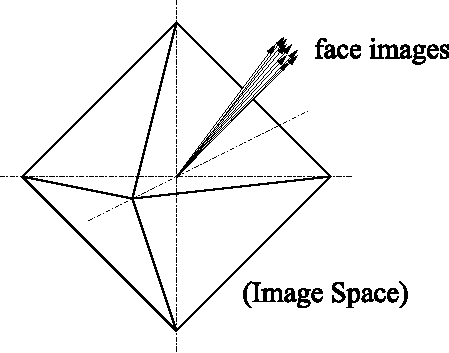
\includegraphics[width=.3\textwidth]{images/bouqet.pdf}\\
\vspace{-.2in}
\end{center}
\begin{itemize}
\item One very promising direction in face recognition research,
{\bf Sparse Representation based Classification (SRC)} [Wright et.\ al. PAMI 2009] achieves state-of-the-art performance on aligned public datasets.
\item This is a solid foundation, but it is incomplete:
	\begin{itemize}
	\item Assumed perfectly aligned images
	\item Assumed a sufficient number of training illuminations taken under different illuminations
\end{itemize}
\end{itemize}
}

\frame{
\frametitle{The Goal of the Research}
{\large I will demonstrate a complete and scalable face recognition system that can handle  {\bf illumination variation, alignment error, and realistic occlusions.}}\\
\vspace{.2in}
This encompases the following major contributions:
\begin{itemize}
\item Determine what {\bf training illuminations} are sufficient and build an {\bf acquisition system} capable of capturing them
\item Design algorithm for {\bf automatically aligning} test images to training images
\item Algorithmic improvements to improve recognition rate
\item Algorithmic improvements to improve recognitieon speed
\item Highly optimized parallel implementations for real-time face recognition
\end{itemize}
}

\subsection{Illumination Model}
\frame{\tableofcontents[currentsection, currentsubsection]}
\frame{\frametitle{Compound effect of alignment and illumination}
\renewcommand{\imagesizestring}{height}
\setlength{\imagesizea}{0.25\textheight}
\setlength{\imagesizeb}{0.15\textheight}
\setlength{\gapsizea}{-0mm}
\begin{tabular}[b]{cc@{}b{.5\textwidth}}
% Example for setting the heights of the images
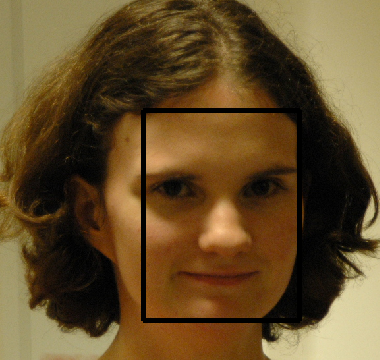
\includegraphics[\imagesizestring=\imagesizea]{figures_cvpr/promo/case1/detector.png}& \hspace{\gapsizea}
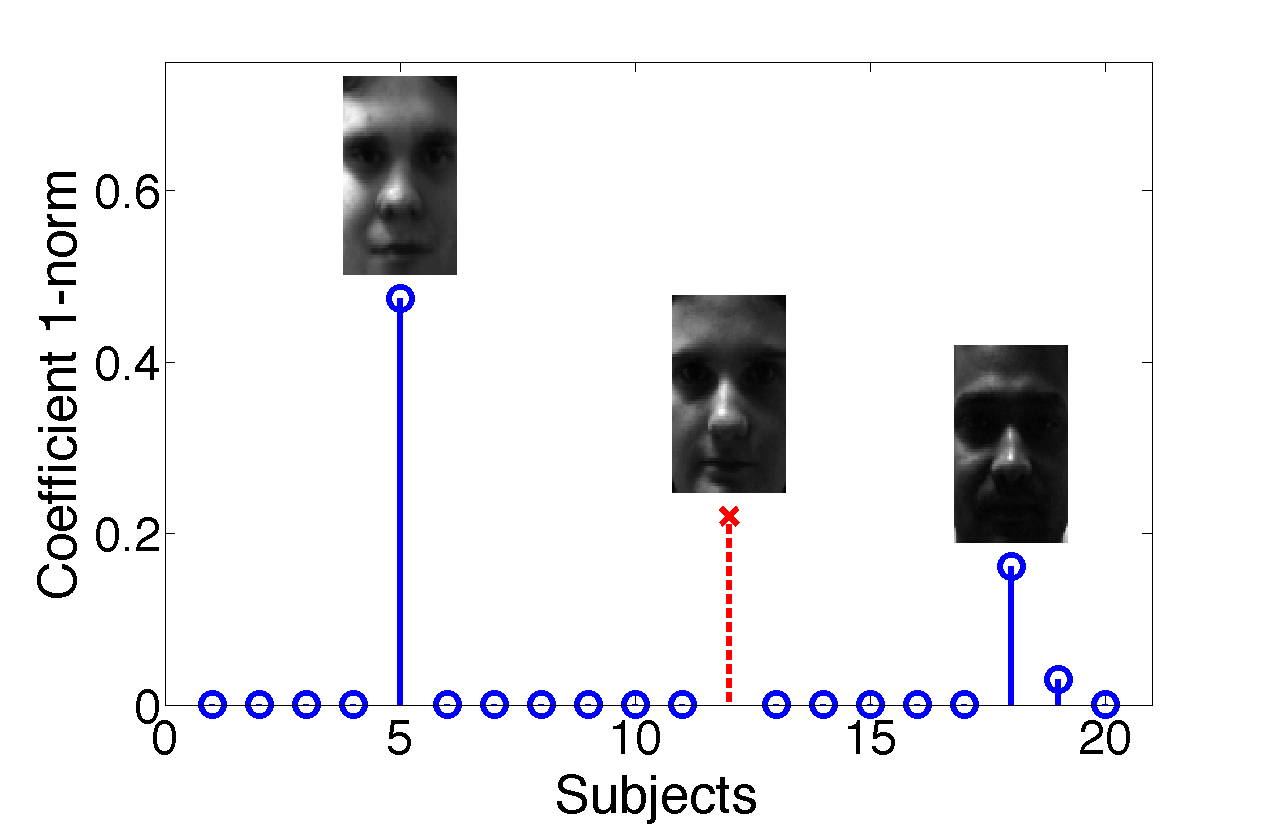
\includegraphics[\imagesizestring=\imagesizea]{figures_cvpr/promo/case1/sci_with_axis_face_case1.png} & 
{\bf Poor alignment}, Sufficient training illuminations \vfill\\
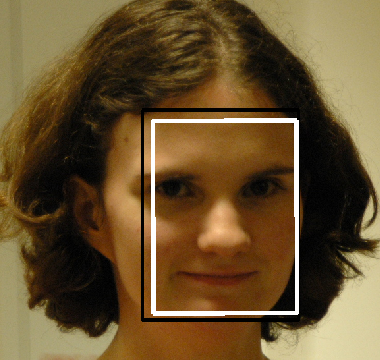
\includegraphics[\imagesizestring=\imagesizea]{figures_cvpr/promo/alignment_and_detector.png}& \hspace{\gapsizea}
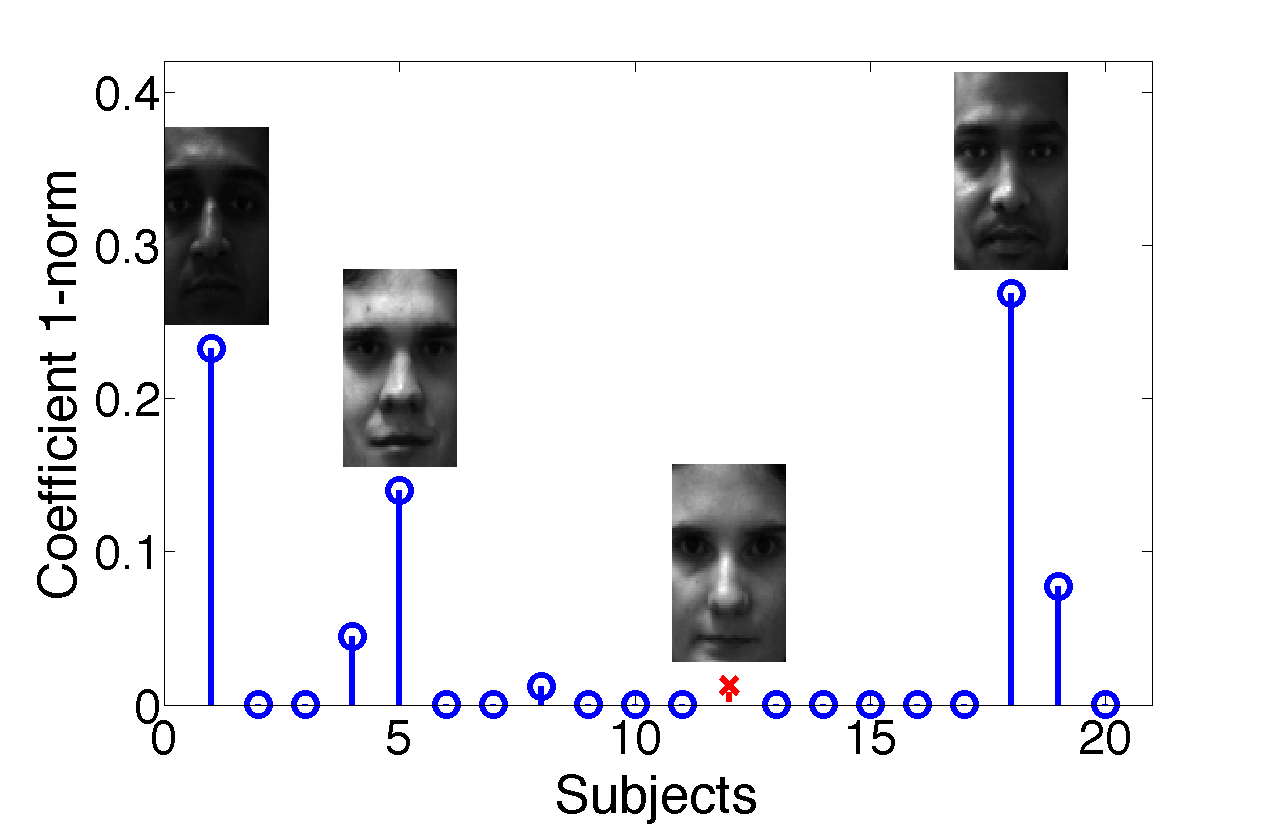
\includegraphics[\imagesizestring=\imagesizea]{figures_cvpr/promo/case2/sci_with_axis_face_case2.png} & 
{{\bf Good alignment}, Insufficient training illuminations}\vfill\\
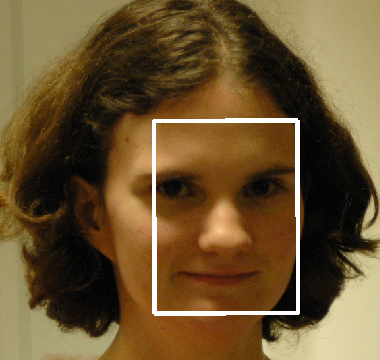
\includegraphics[\imagesizestring=\imagesizea]{figures_cvpr/promo/case3/alignment.png} & \hspace{\gapsizea}
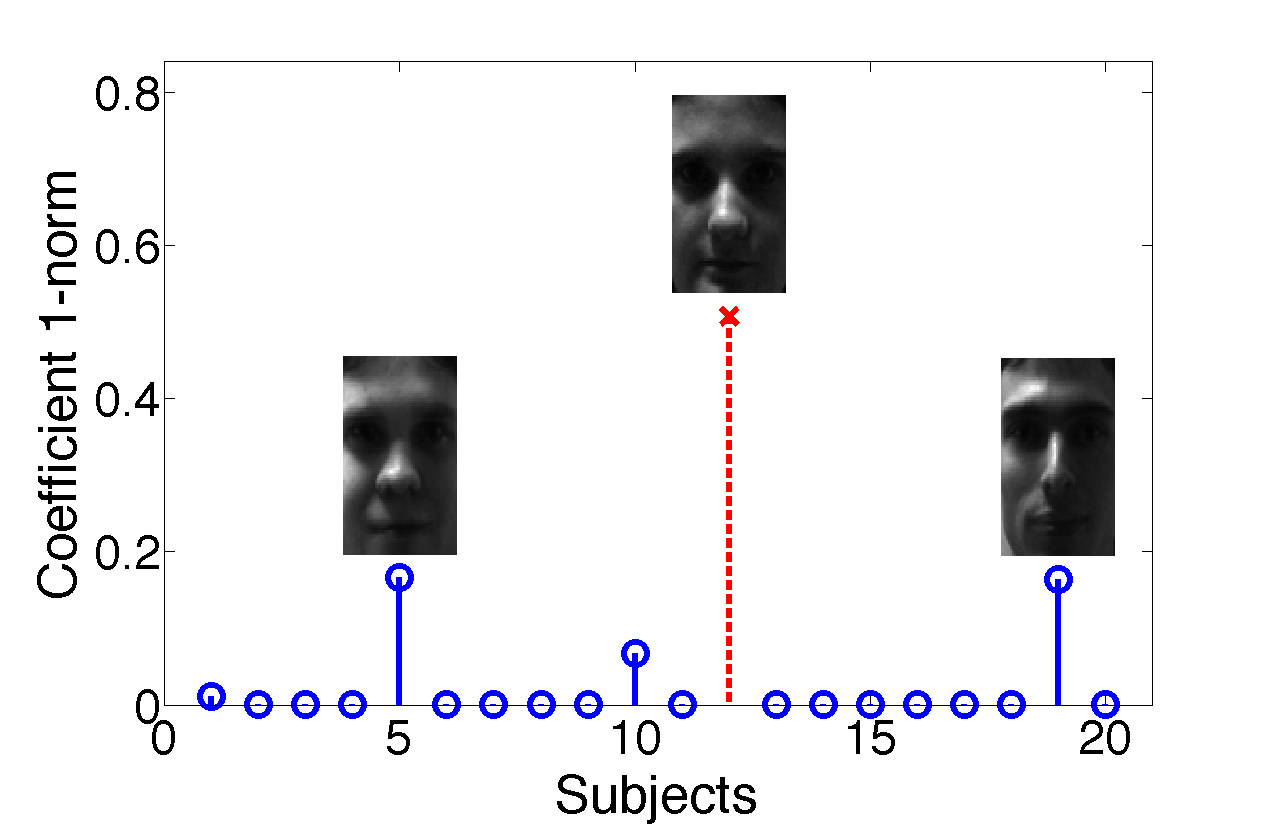
\includegraphics[\imagesizestring=\imagesizea]{figures_cvpr/promo/case3/sci_with_axis_face_case3.png} &
{{\bf Good alignment}, Sufficient training illuminations}\vfill
\end{tabular}
}


%\frame{
%\frametitle{Linear Illumination Models}
%\hspace{.1\textwidth}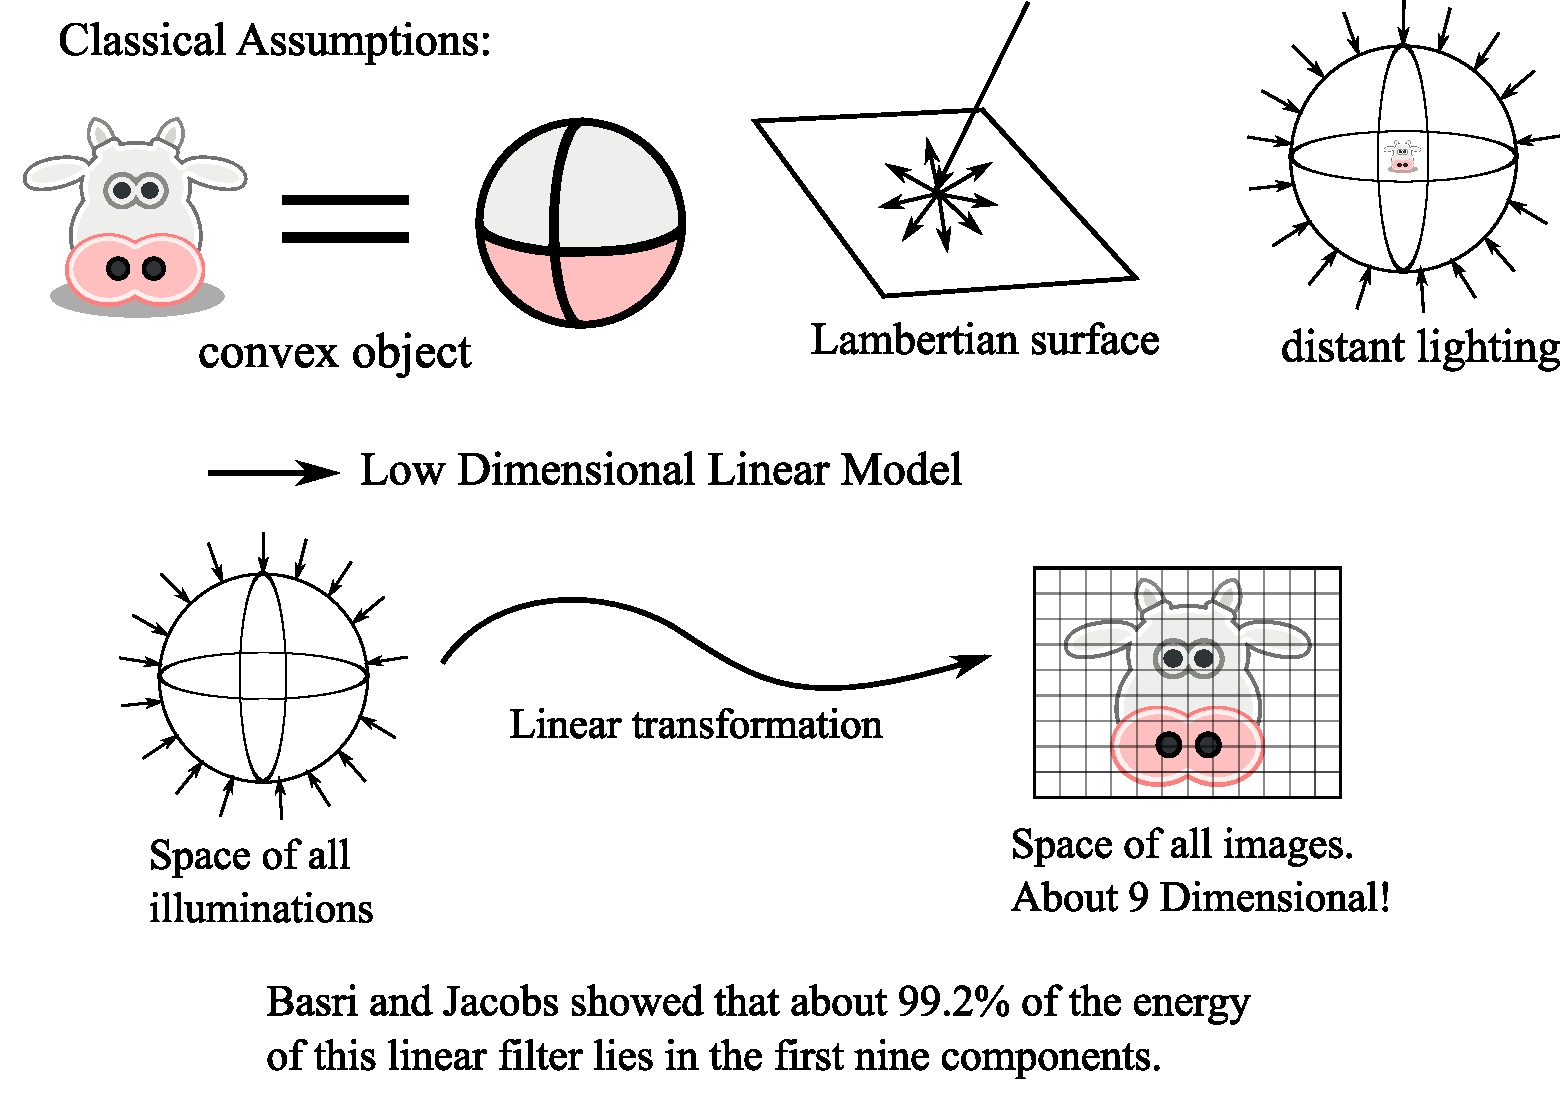
\includegraphics[height=0.8\textheight]{images/linear_illumination_model.pdf}
%}

\frame{
\frametitle{Linear Illumination Models}
\vspace{-5mm}\begin{center}
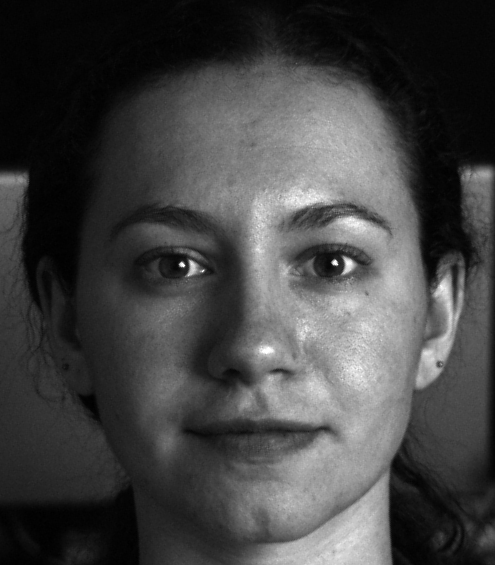
\includegraphics[width=0.3\textwidth]{images/shadow_example}
\end{center}\vspace{-5mm}
\begin{itemize}
\item Despite Shadowing and Specularities Images still linear WRT illumination
\item We can make Shadows and Specularities our Friends rather than our Enemies
\item {\em Experimentally} determine which training illuminations needed
\end{itemize}
}

\frame{
\frametitle{Acquisition System}
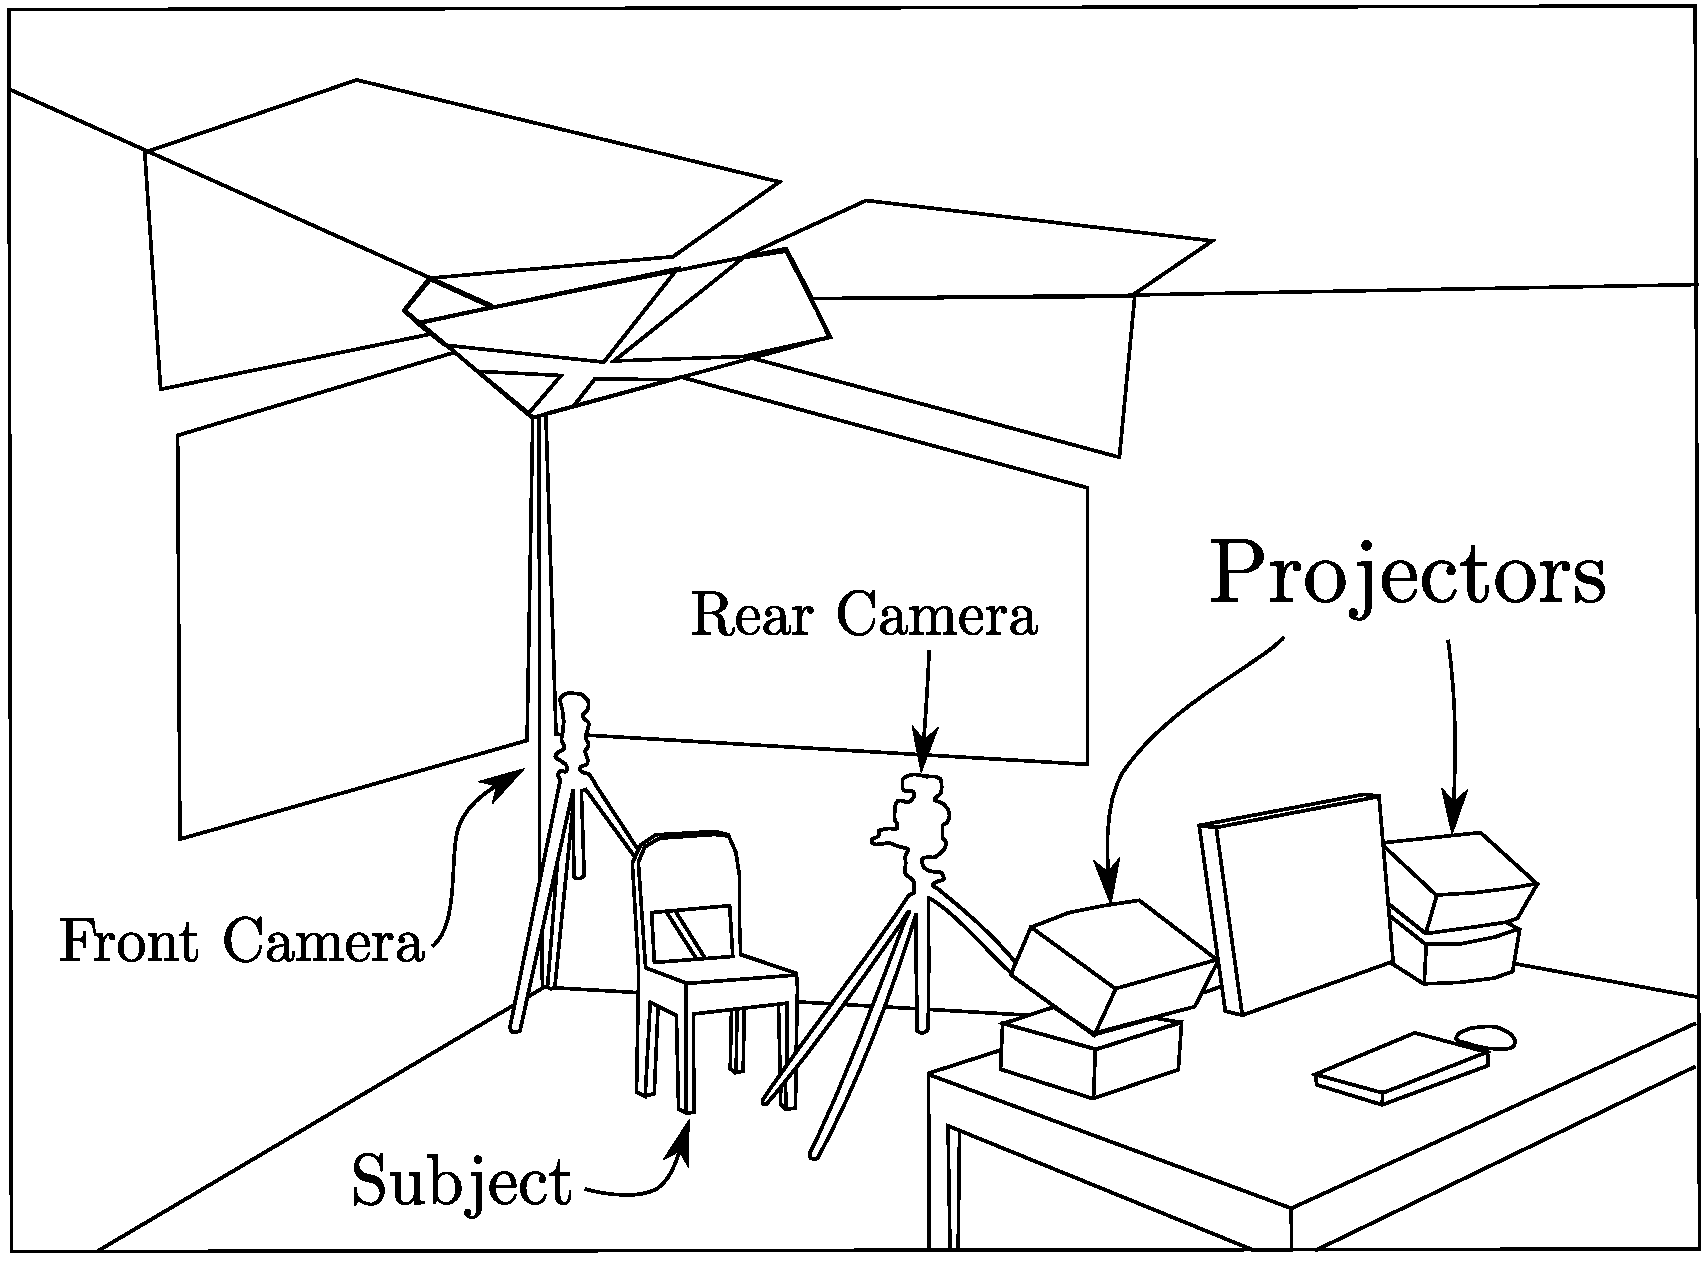
\includegraphics[width=0.3\textwidth]{images/camera_rig_drawings/perspective.pdf}

Projector-Based System:
\begin{itemize}
\item Easy to re-configure projector geometry
\item Trivial to change illumination patterns
\item Easier to construct and deploy
\item Very complete angular illumination coverage
\end{itemize}
}

\frame{
\frametitle{Training Illumination Rig}
\begin{columns}
\begin{column}{.5\textwidth}
\begin{center}
Side View\\
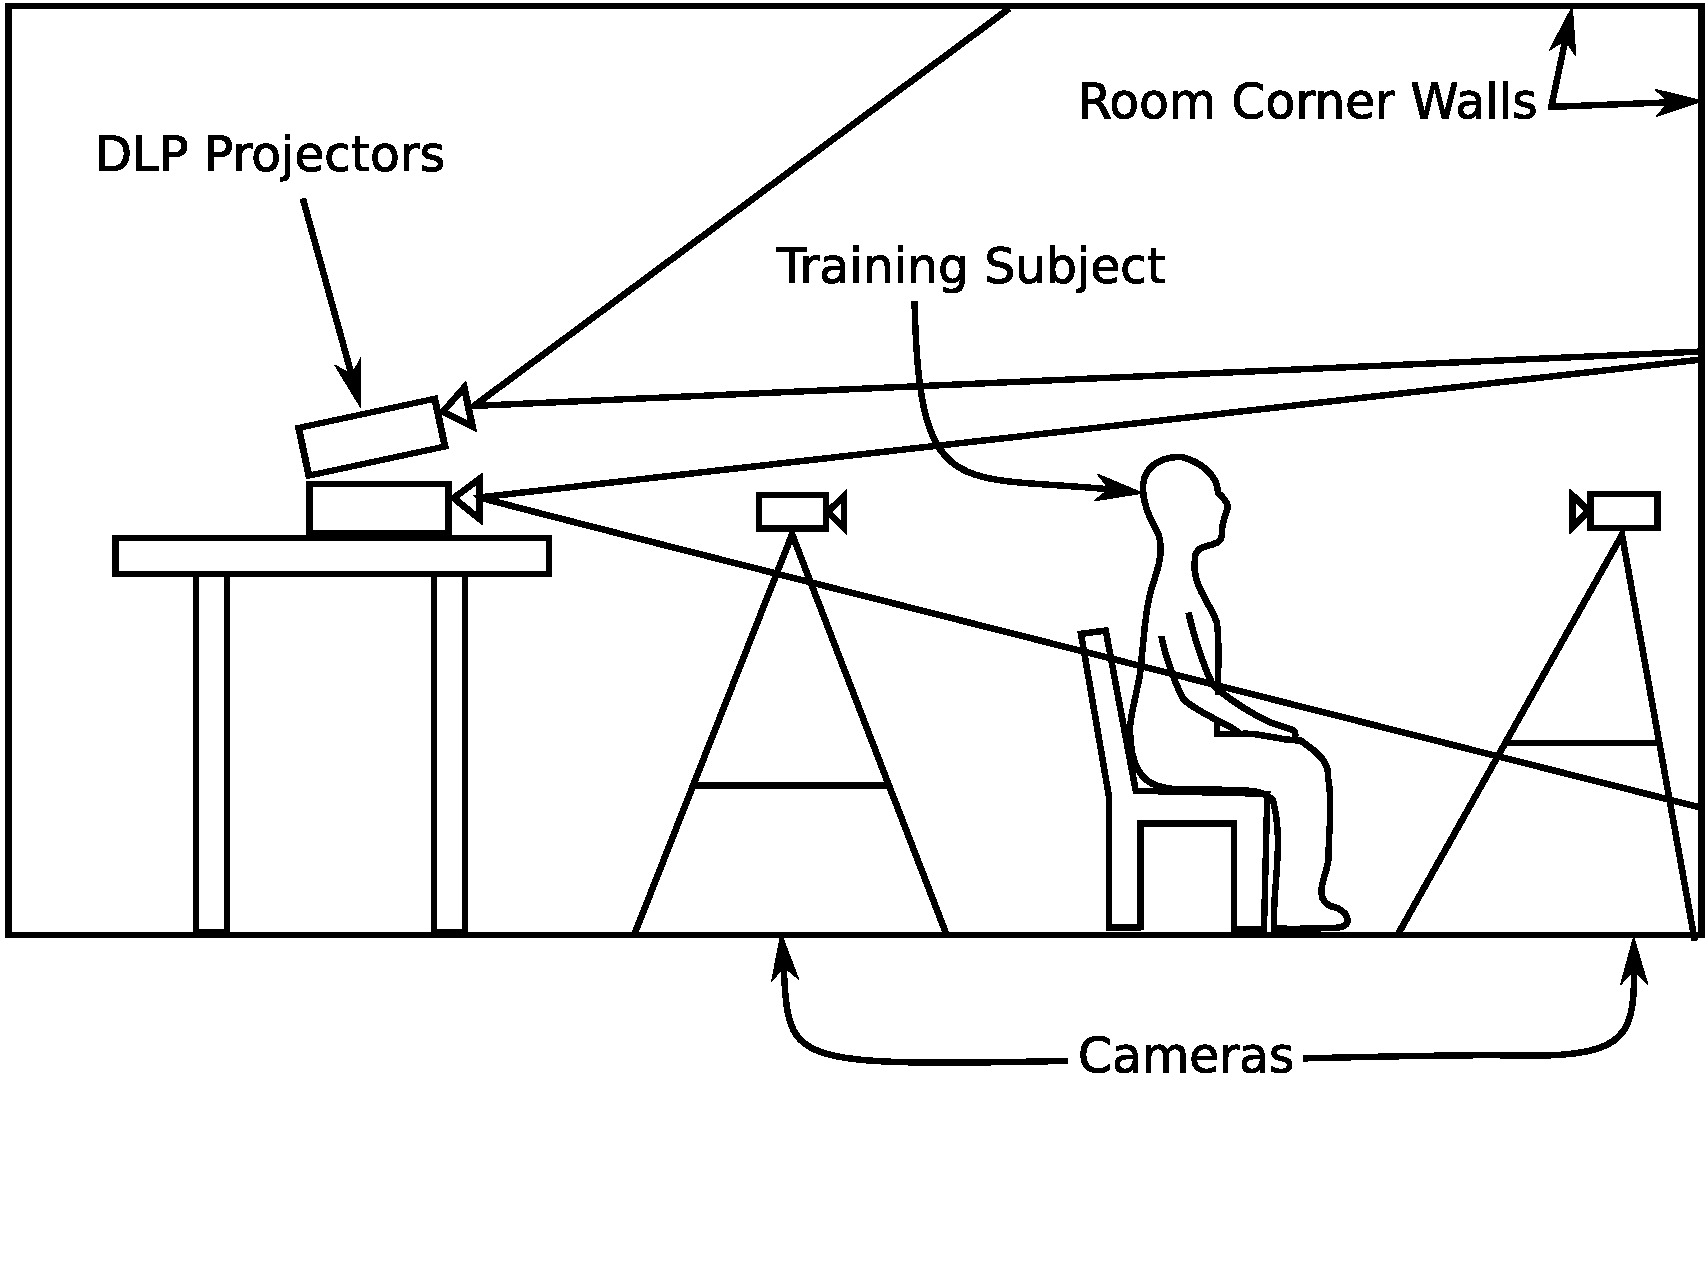
\includegraphics[width=\textwidth]{images/camera_rig_drawings/coverage_side.pdf}
\end{center}
\end{column}
\begin{column}{.5\textwidth}
\begin{center}
Top View\\
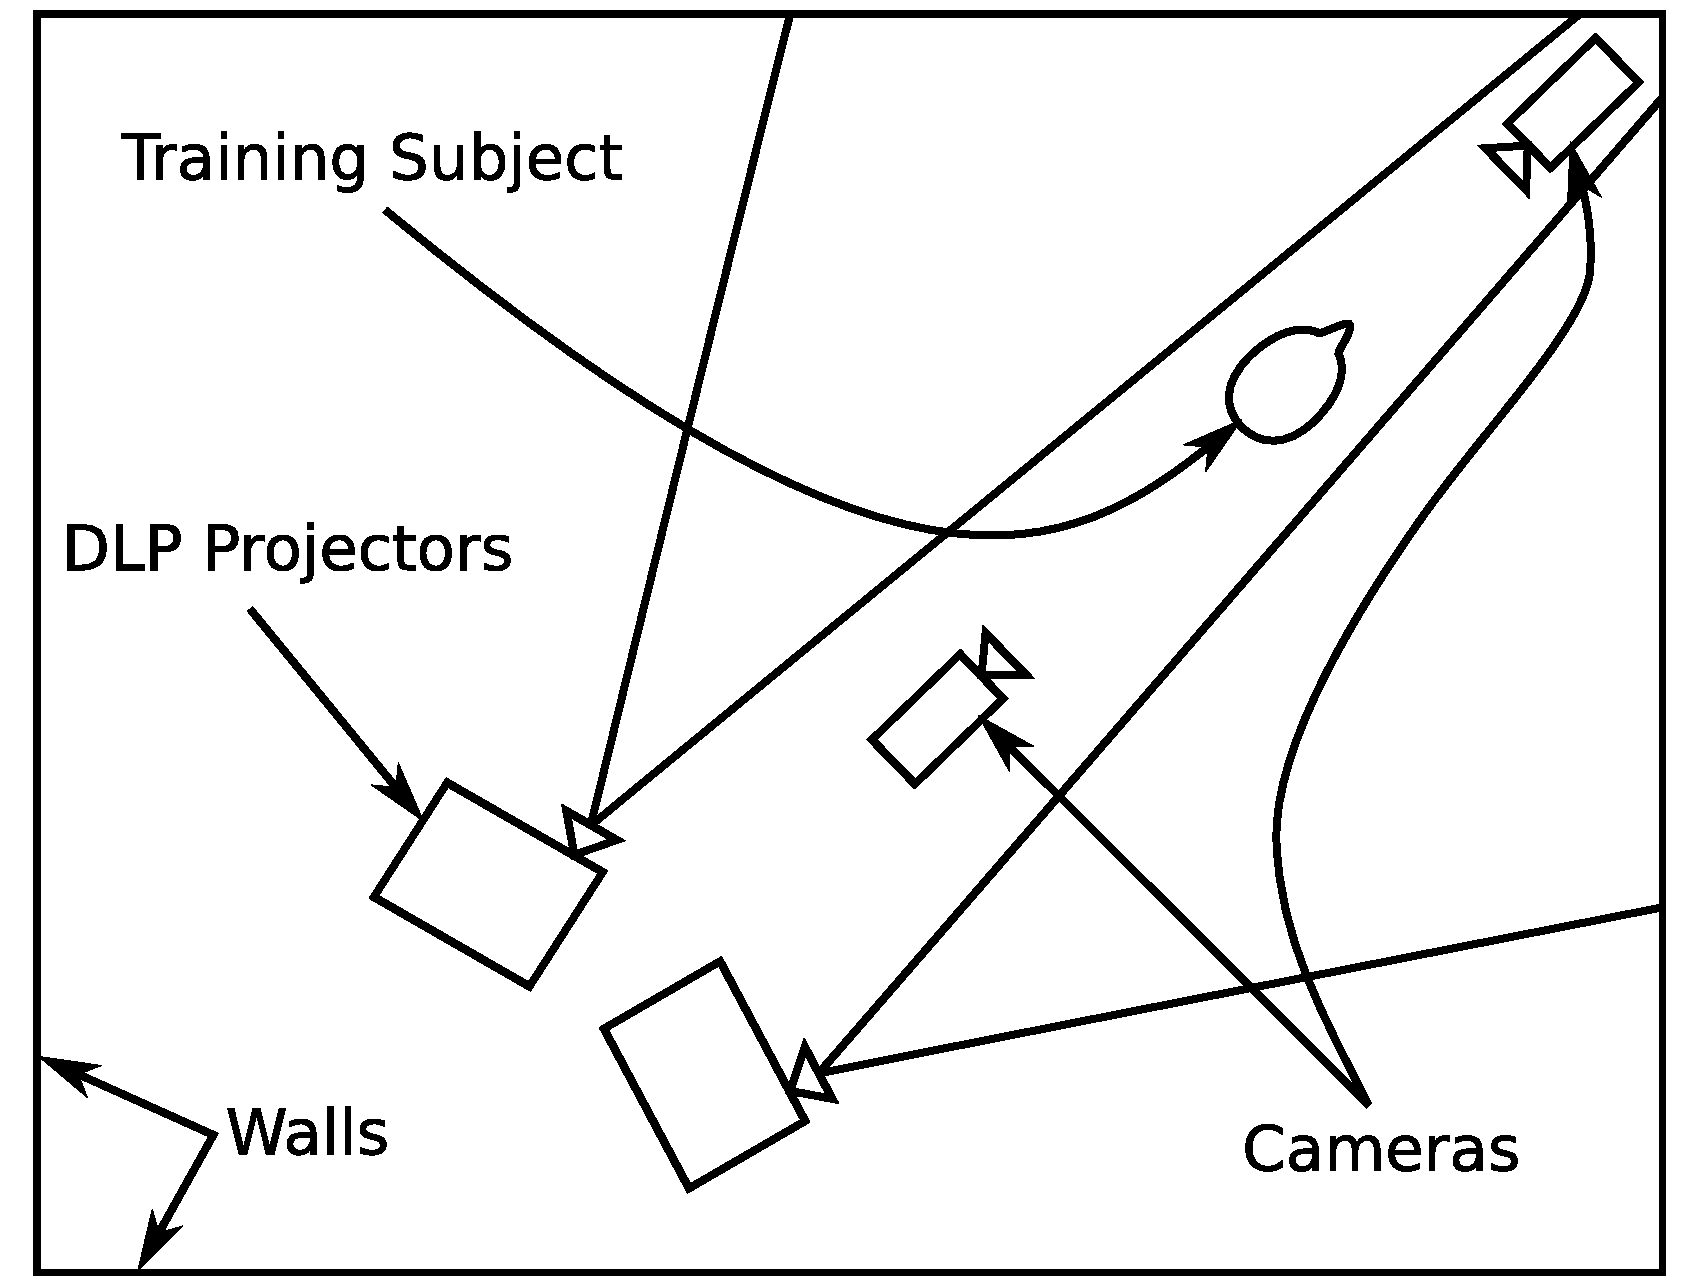
\includegraphics[width=\textwidth]{images/camera_rig_drawings/coverage_top.pdf}
\end{center}
\end{column}
\end{columns}
}

\frame{
\renewcommand{\imagesizestring}{height}
\setlength{\imagesizea}{0.41\textheight}
\frametitle{Experimentally Motivated Illumination Set}
\begin{tabular}{cc}
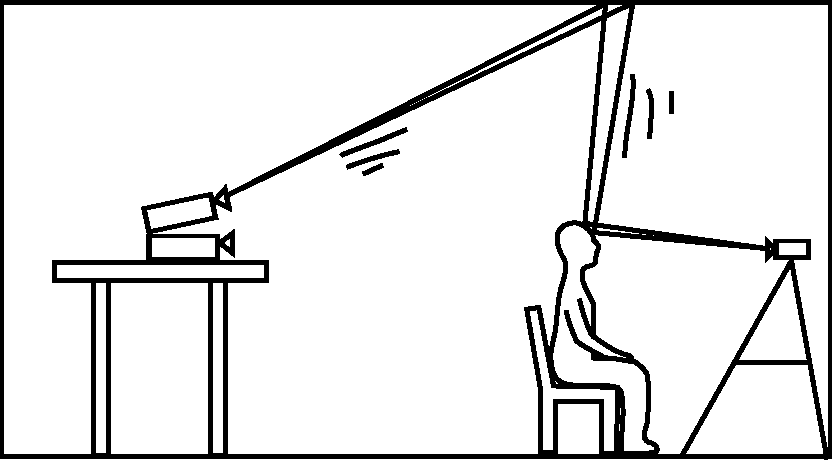
\includegraphics[\imagesizestring = \imagesizea]{images/camera_rig_drawings/side_front.pdf} & 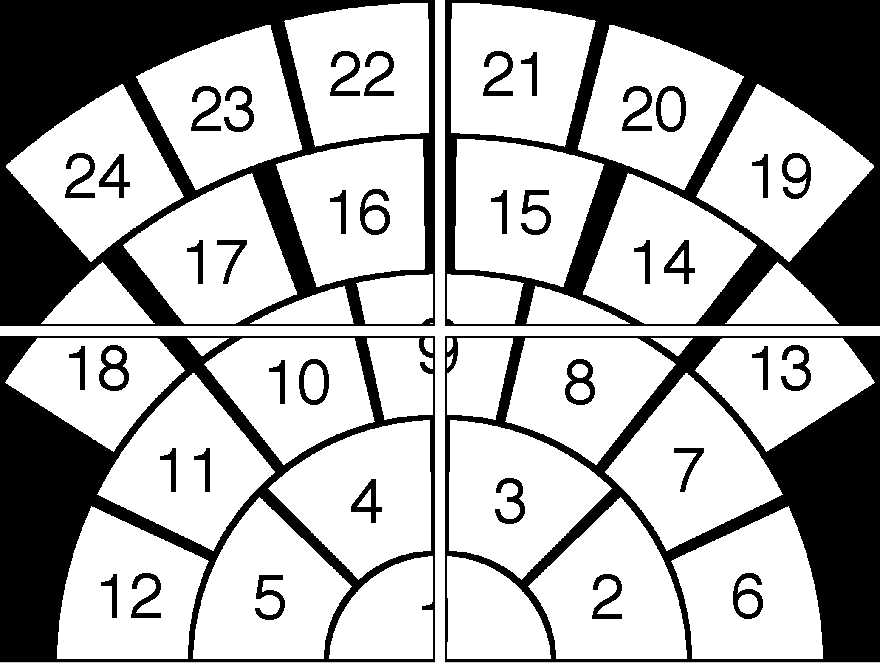
\includegraphics[\imagesizestring = \imagesizea]{images/illuminations/front.png}\\
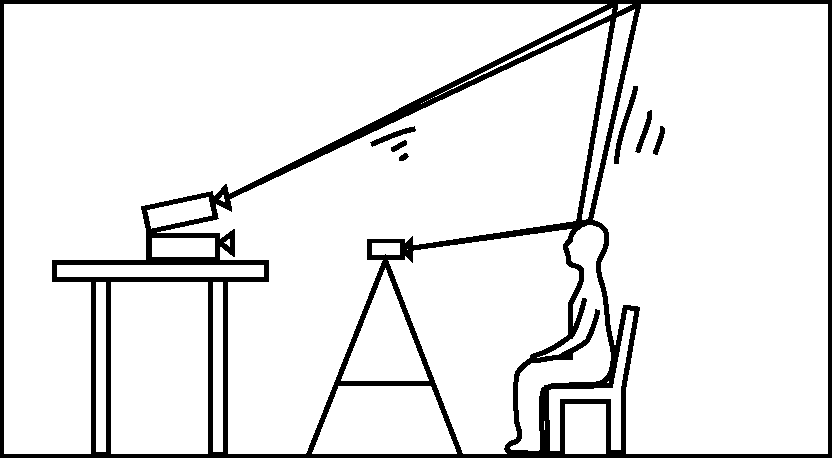
\includegraphics[\imagesizestring = \imagesizea]{images/camera_rig_drawings/side_back.pdf} & 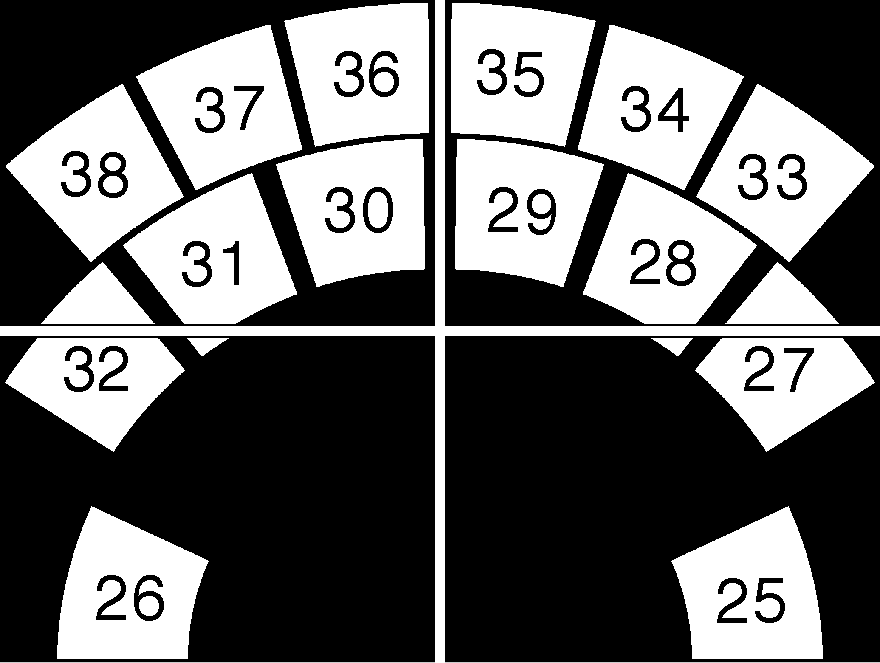
\includegraphics[\imagesizestring = \imagesizea]{images/illuminations/back.png}
\end{tabular}
}

%\frame{\frametitle{Sample Training Images, Originals}
%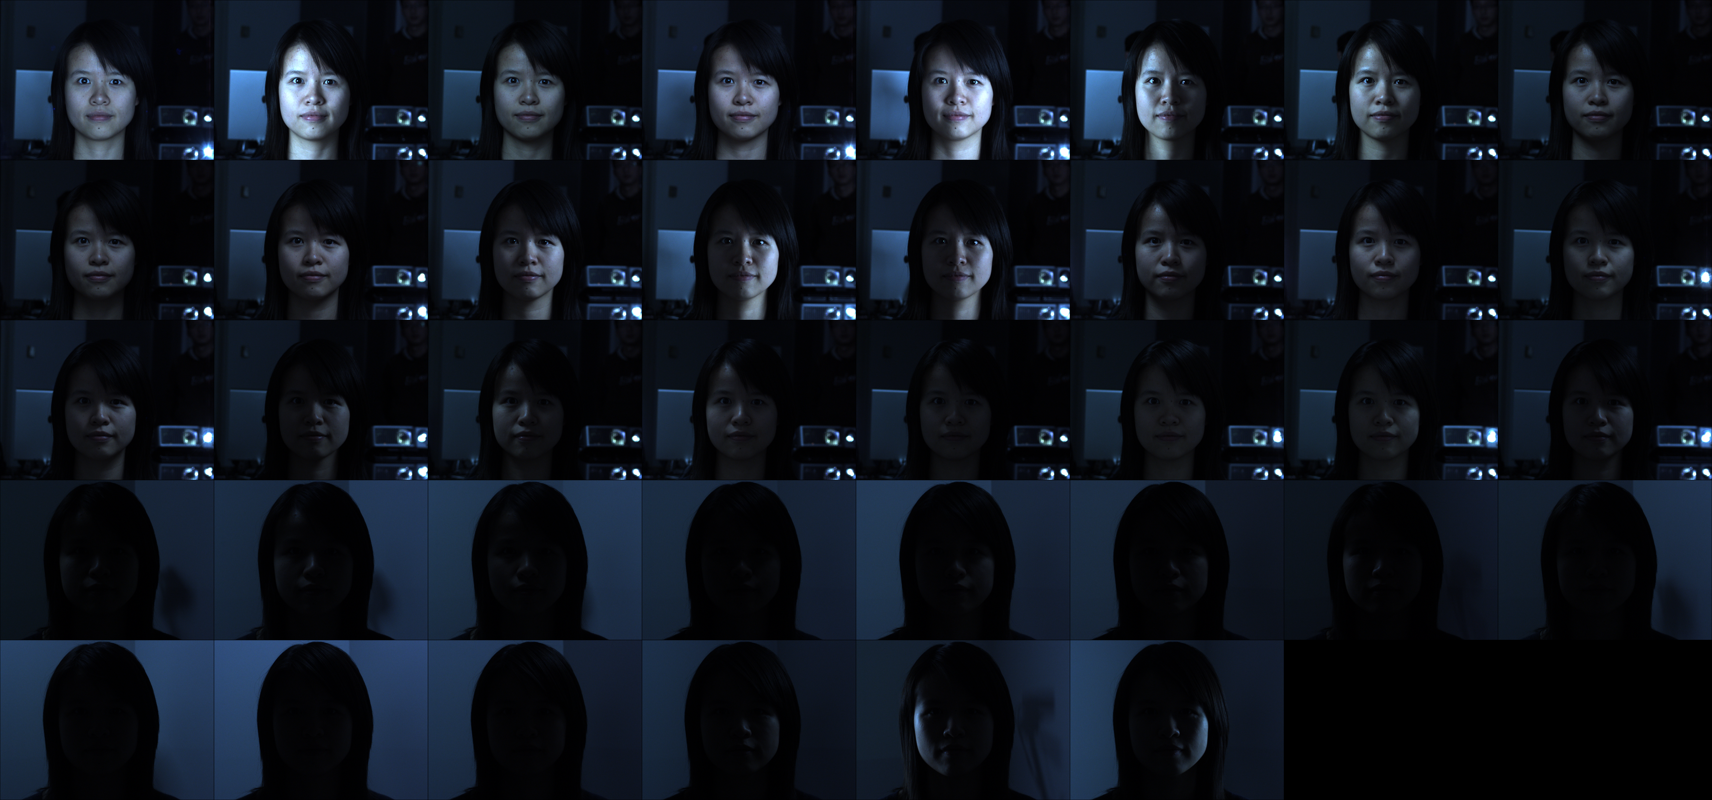
\includegraphics[width=\textwidth]{images/training_contact_sheet.png}
%}

\subsection{Alignment}
\frame{\tableofcontents[currentsection, currentsubsection]}
%\frame{\frametitle{Compound effect of alignment and illumination}
\renewcommand{\imagesizestring}{height}
\setlength{\imagesizea}{0.25\textheight}
\setlength{\imagesizeb}{0.15\textheight}
\setlength{\gapsizea}{-0mm}
\begin{tabular}[b]{cc@{}b{.5\textwidth}}
% Example for setting the heights of the images
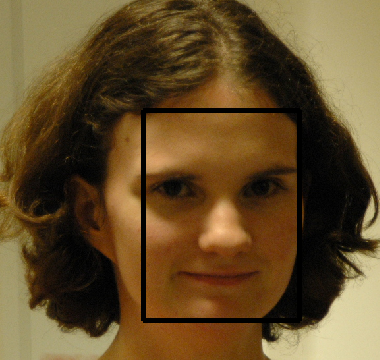
\includegraphics[\imagesizestring=\imagesizea]{figures_cvpr/promo/case1/detector.png}& \hspace{\gapsizea}
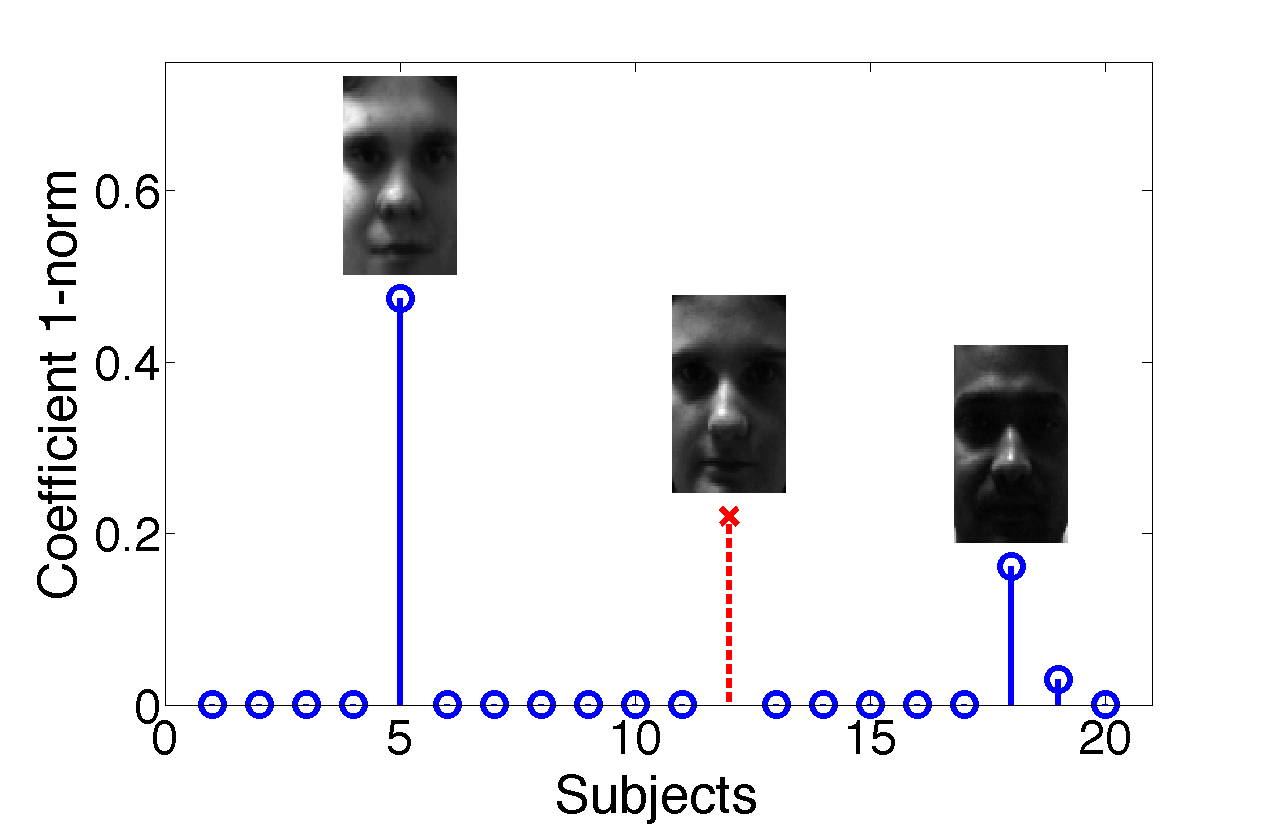
\includegraphics[\imagesizestring=\imagesizea]{figures_cvpr/promo/case1/sci_with_axis_face_case1.png} & 
{\bf Poor alignment}, Sufficient training illuminations \vfill\\
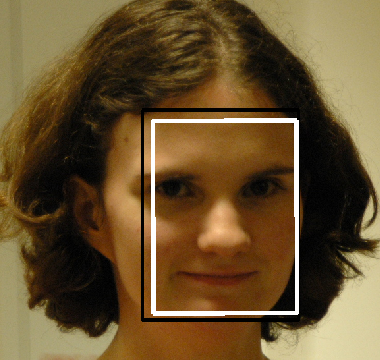
\includegraphics[\imagesizestring=\imagesizea]{figures_cvpr/promo/alignment_and_detector.png}& \hspace{\gapsizea}
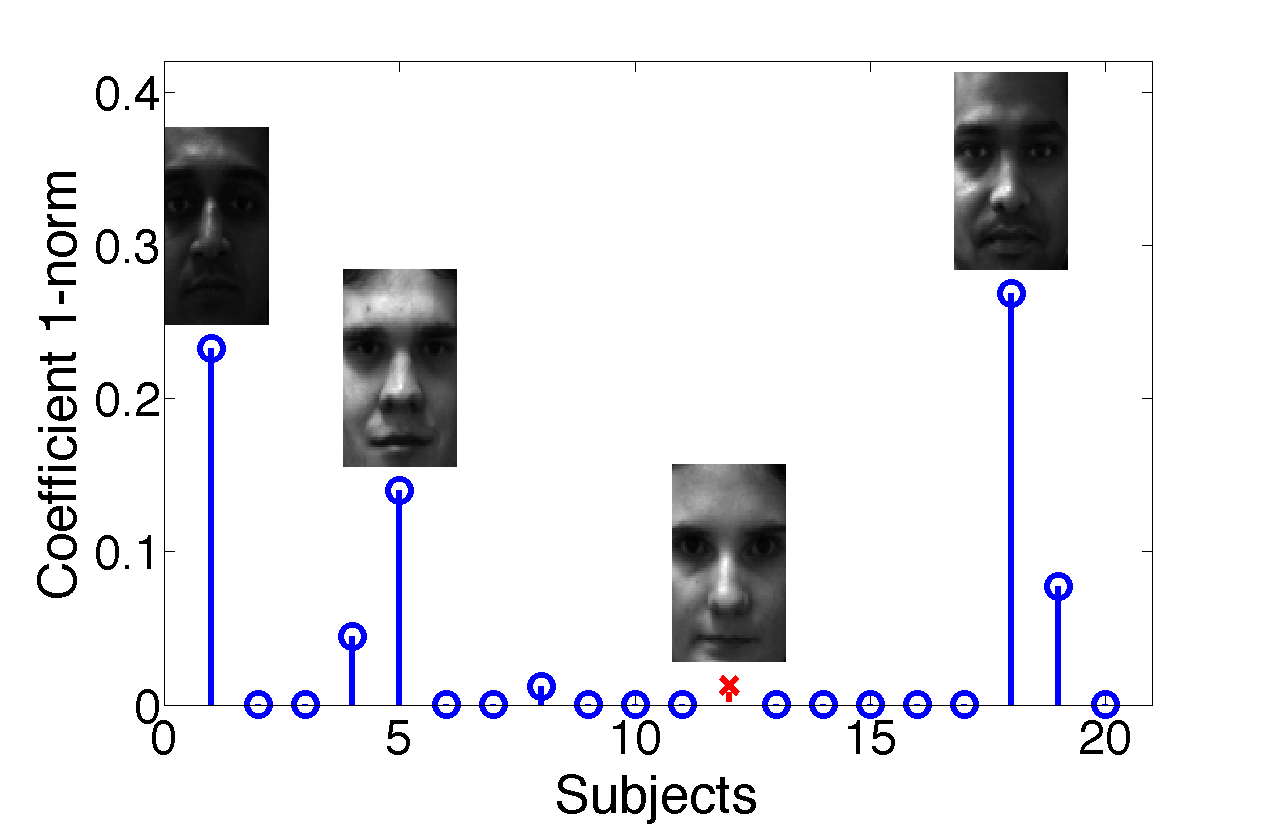
\includegraphics[\imagesizestring=\imagesizea]{figures_cvpr/promo/case2/sci_with_axis_face_case2.png} & 
{{\bf Good alignment}, Insufficient training illuminations}\vfill\\
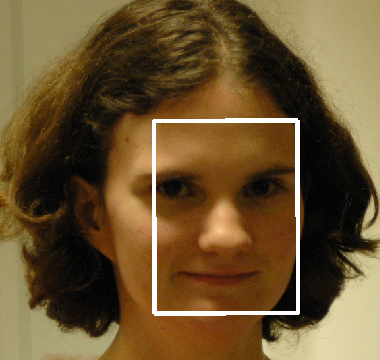
\includegraphics[\imagesizestring=\imagesizea]{figures_cvpr/promo/case3/alignment.png} & \hspace{\gapsizea}
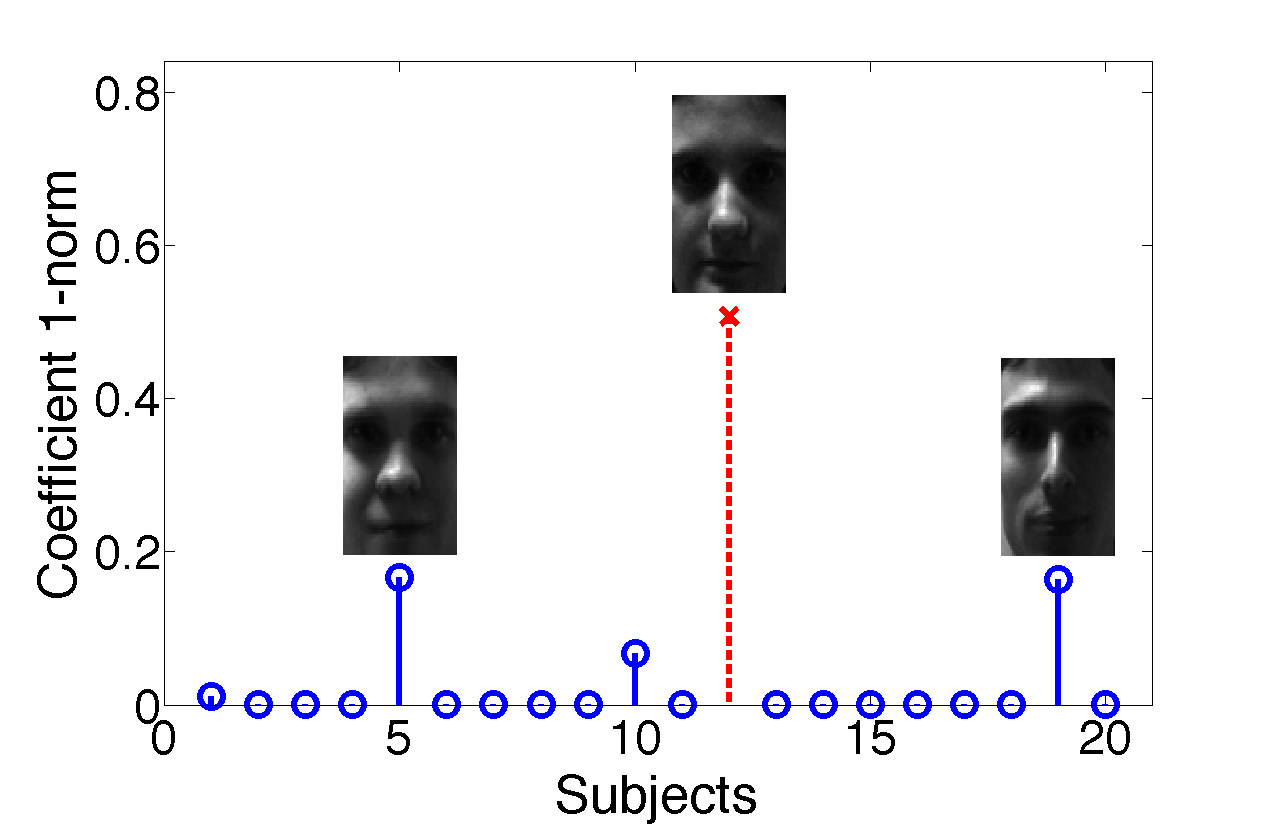
\includegraphics[\imagesizestring=\imagesizea]{figures_cvpr/promo/case3/sci_with_axis_face_case3.png} &
{{\bf Good alignment}, Sufficient training illuminations}\vfill
\end{tabular}
}


\frame{
\frametitle{Image Embedding}
\vspace{-3mm}
\begin{center}
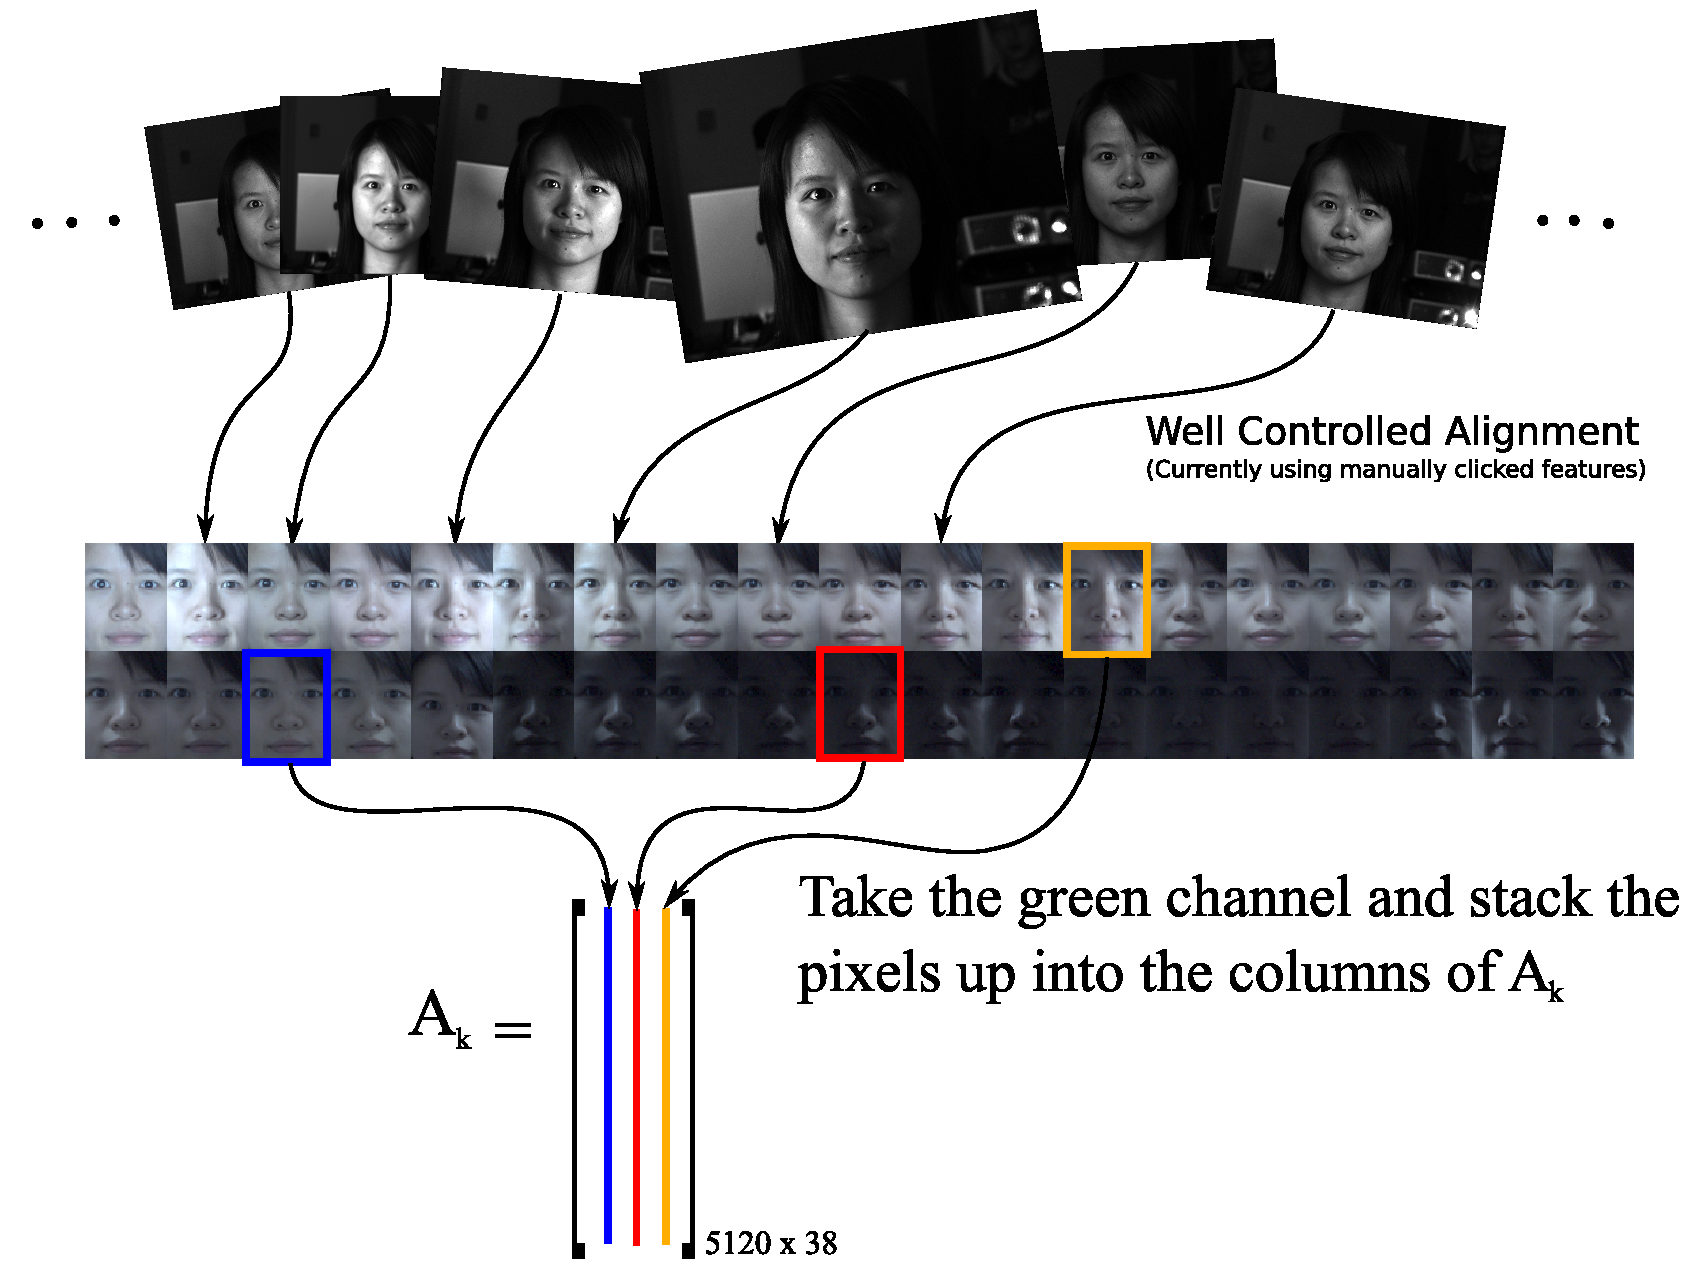
\includegraphics[width=.50\textwidth]{figures_embedding/training_embedding.pdf}\\
$A = [ A_1 \mid A_2 \mid \dots \mid A_K ] \in \Re^{m \times n}$
\end{center}
}


\frame{
\frametitle{Recognition Pipeline}
\begin{equation*}
(\hat \x, \hat \e,\hat \tau_i) = \argmin{\x,\e,\tau_i \in T} \| \e \|_1 \quad \subj \quad \y \circ \tau_i = A_i \x + \e
\end{equation*}
\begin{center}
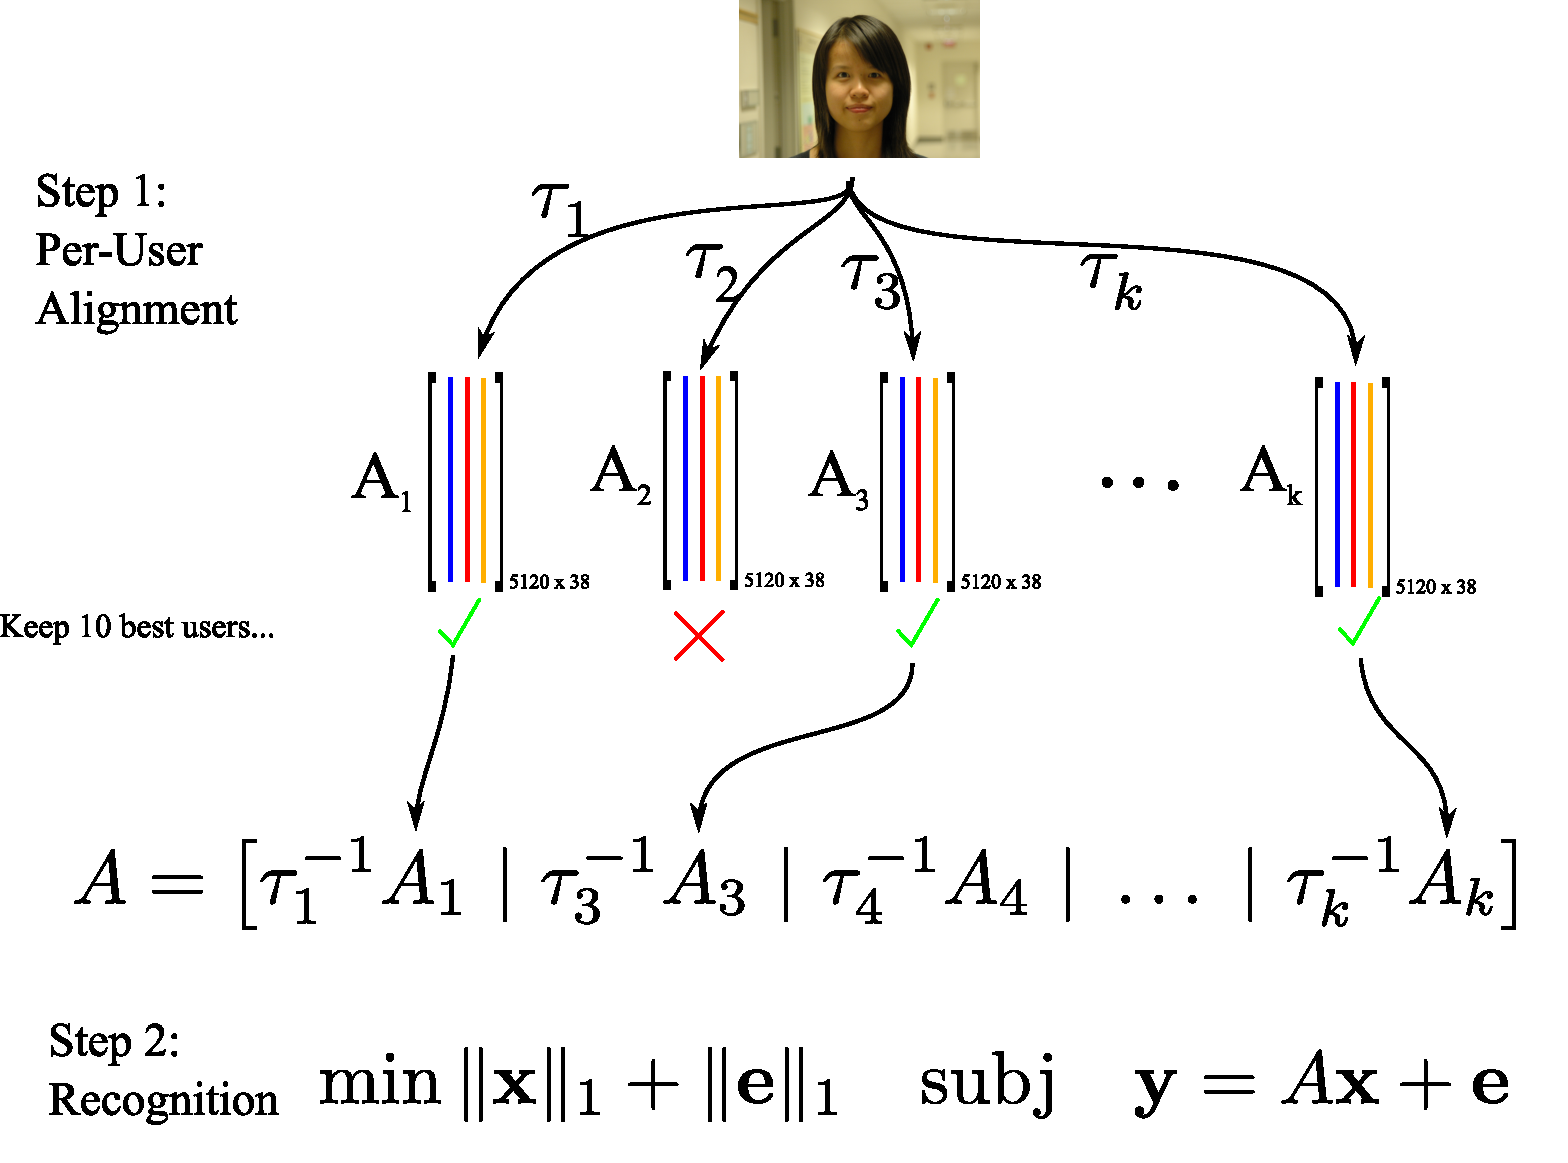
\includegraphics[width=.75\textwidth]{figures_embedding/pipeline.pdf}
\end{center}
}


%\frame{\frametitle{Alignment Examples}
%$\ell^1$ and $\ell^2$ minimization alignment comparison
%\begin{columns}
%\begin{column}{0.5\textwidth}
%\renewcommand{\imagesizestring}{height}
%\setlength{\imagesizea}{0.2\textheight}
%\begin{tabular}[t]{@{}c@{}c@{}c@{}c@{}m{.2\textwidth}}
%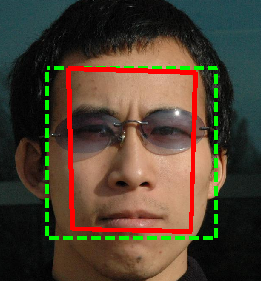
\includegraphics[\imagesizestring=\imagesizea]{figures_cvpr/L1_cropped} &
%
\includegraphics[\imagesizestring=\imagesizea]{figures_cvpr/y_warp_L1} &
%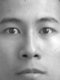
\includegraphics[\imagesizestring=\imagesizea]{figures_cvpr/y_hat_L1} &
%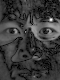
\includegraphics[\imagesizestring=\imagesizea]{figures_cvpr/e_L1} &
%$\|\e\|_1$\\[-.05in]
%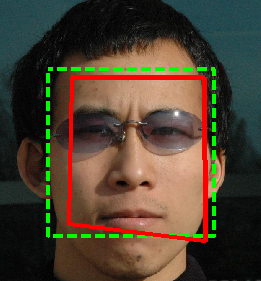
\includegraphics[\imagesizestring=\imagesizea]{figures_cvpr/L2_cropped} &
%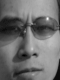
\includegraphics[\imagesizestring=\imagesizea]{figures_cvpr/y_warp_L2} &
%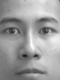
\includegraphics[\imagesizestring=\imagesizea]{figures_cvpr/y_hat_L2} &
%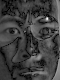
\includegraphics[\imagesizestring=\imagesizea]{figures_cvpr/e_L2} &
%$\|\e\|_2$ \\[-.1in]
%{\tiny Face Boundary} & {\tiny Aligned Test} & {\tiny Reconstruction} & {\tiny $|$Error$|$}
%\end{tabular}
%\end{column}
%\begin{column}{0.5\textwidth}
%\renewcommand{\imagesizestring}{height}
%\setlength{\imagesizea}{0.2\textheight}
%Alignment tolerance for out-of-plane pose variation
%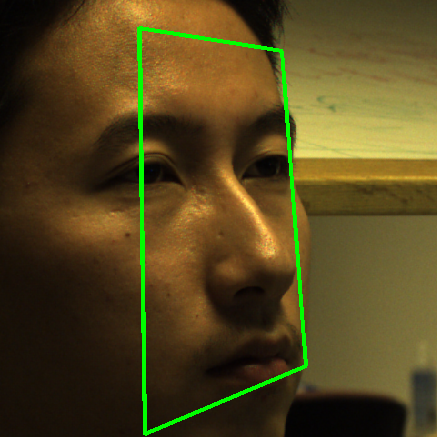
\includegraphics[\imagesizestring=\imagesizea]{figures_cvpr/21}
%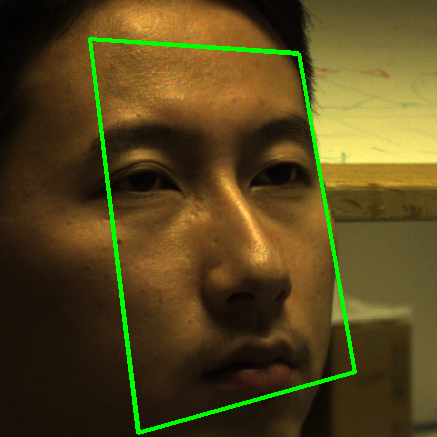
\includegraphics[\imagesizestring=\imagesizea]{figures_cvpr/19}
%
\includegraphics[\imagesizestring=\imagesizea]{figures_cvpr/17}
%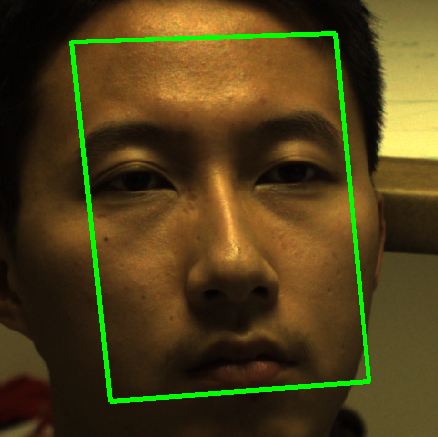
\includegraphics[\imagesizestring=\imagesizea]{figures_cvpr/15}
%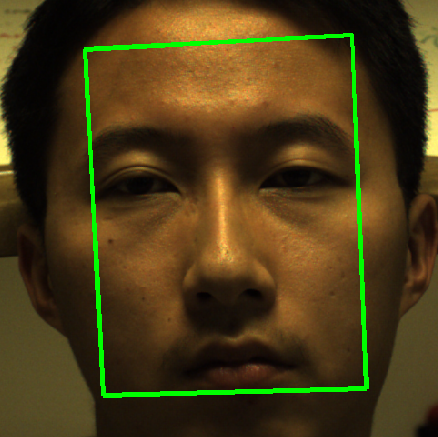
\includegraphics[\imagesizestring=\imagesizea]{figures_cvpr/13}\\
%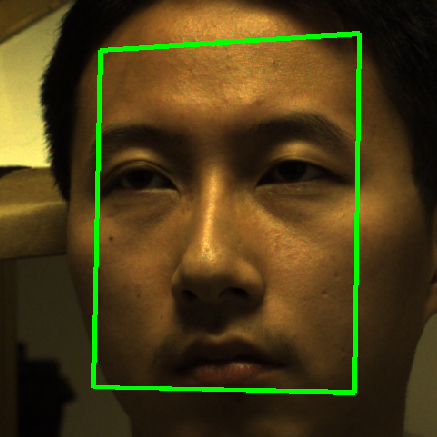
\includegraphics[\imagesizestring=\imagesizea]{figures_cvpr/11}
%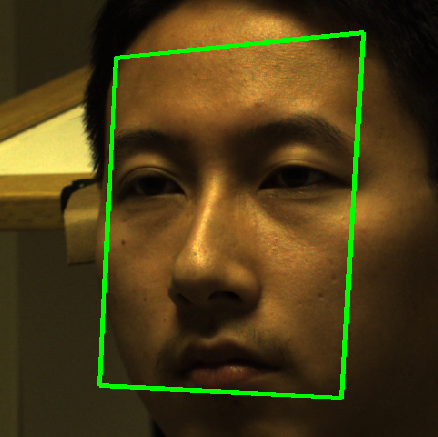
\includegraphics[\imagesizestring=\imagesizea]{figures_cvpr/09}
%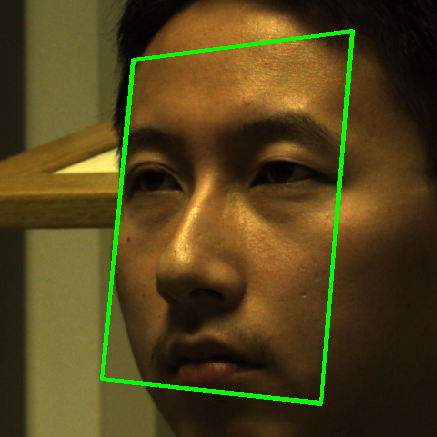
\includegraphics[\imagesizestring=\imagesizea]{figures_cvpr/7}
%
\includegraphics[\imagesizestring=\imagesizea]{figures_cvpr/5}
%
\includegraphics[\imagesizestring=\imagesizea]{figures_cvpr/3}\\
%Alignment using a projective transformation works up to about $45^{\circ}$.
%\end{column}
%\end{columns}
%}


\renewcommand{\imagesizestring}{height}
\setlength{\imagesizea}{0.36\textheight}
\setlength{\gapsizea}{-0mm}
\frame{\frametitle{Alignment region of attraction}
%\begin{tabular}{cc}
\begin{center}
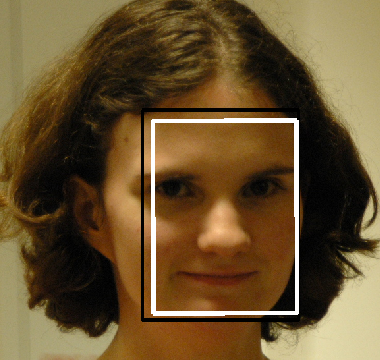
\includegraphics[\imagesizestring=\imagesizea]{figures_cvpr/promo/alignment_and_detector.png}
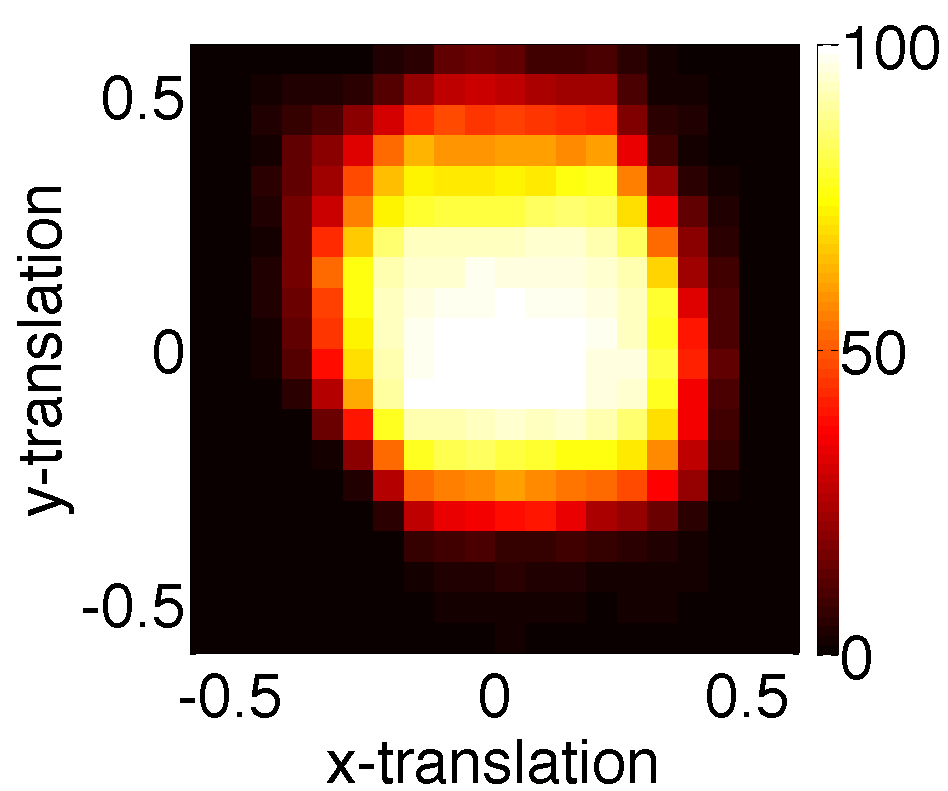
\includegraphics[\imagesizestring= \imagesizea]{figures_cvpr/translation_fig3.png}
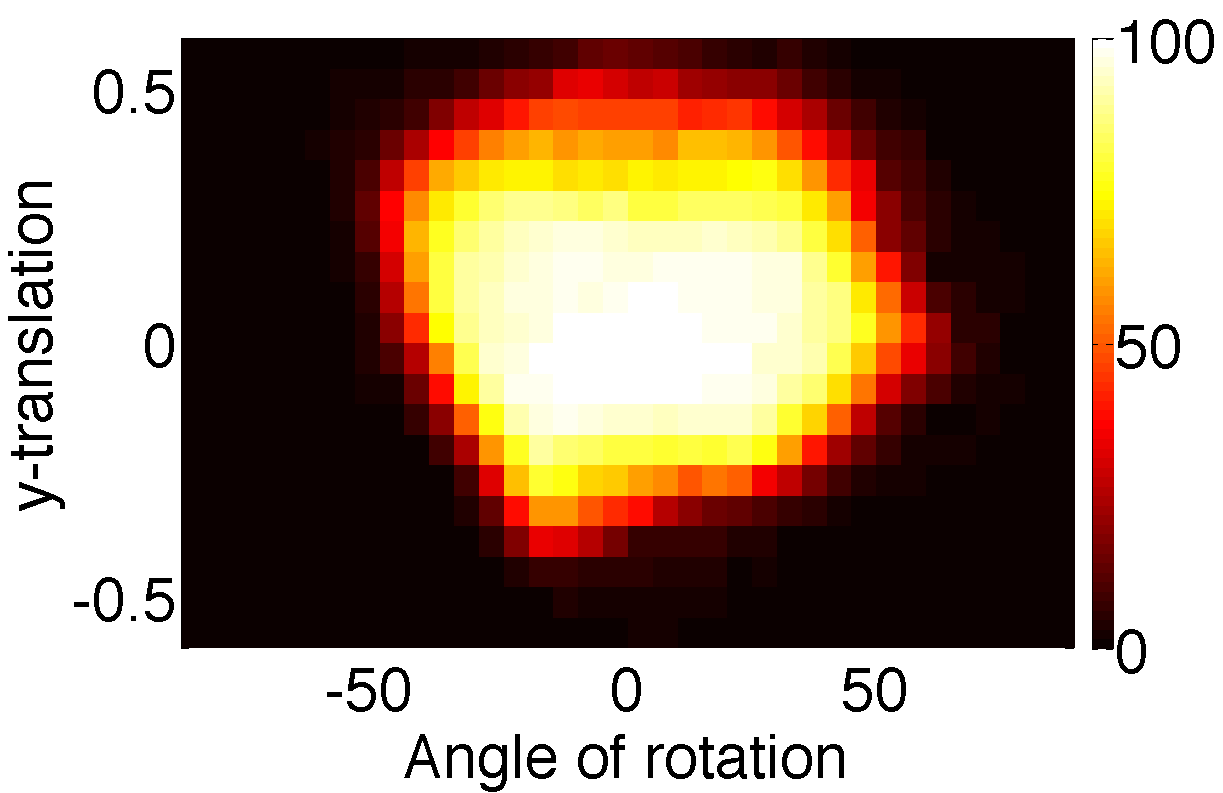
\includegraphics[\imagesizestring= \imagesizea]{figures_cvpr/translation_rotation_fig1.png}
\end{center}
%\end{tabular}
\vspace{0mm}
{\tiny
\begin{itemize}
\item Translation is expressed as a fraction of outer eye corner distance.
\item In-plane rotation is expressed in degrees. 
\item Probability of convergence from synthetic transformations to hand-clicked ground truth
\item Training: CMU Multi-PIE, 120 subjects, 11 illuminations, session 2.  Re-sampled to $60 \times 80$ pixels.
\item Testing: 1 new illumination from session 3
\item Viola Jones' face detector average error on this data set falls safely within our region of attraction
\end{itemize}}
}


%\frame{\frametitle{Alignment Examples}
%{\footnotesize
%\vspace{-.1in}
%Comparison of $\ell^1$ and $\ell^2$ minimization:
%\renewcommand{\imagesizestring}{height}
%\setlength{\imagesizea}{0.15\textheight}
%\vspace{-.05in}
%\begin{center}
%\begin{tabular}[t]{b{.3in}cccc}
%$\min \|\e\|_2$\vfill &
%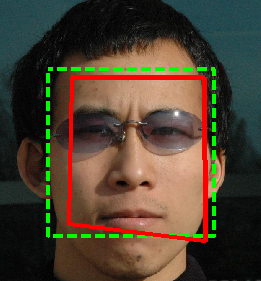
\includegraphics[\imagesizestring=\imagesizea]{figures_cvpr/L2_cropped} &
%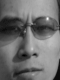
\includegraphics[\imagesizestring=\imagesizea]{figures_cvpr/y_warp_L2} &
%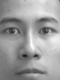
\includegraphics[\imagesizestring=\imagesizea]{figures_cvpr/y_hat_L2} &
%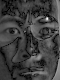
\includegraphics[\imagesizestring=\imagesizea]{figures_cvpr/e_L2} \\
%$\min \|\e\|_1$\vfill &
%\includegraphics[\imagesizestring=\imagesizea]{figures_cvpr/L1_cropped} &
%\includegraphics[\imagesizestring=\imagesizea]{figures_cvpr/y_warp_L1} &
%\includegraphics[\imagesizestring=\imagesizea]{figures_cvpr/y_hat_L1} &
%\includegraphics[\imagesizestring=\imagesizea]{figures_cvpr/e_L1} \\
%& {\tiny Face Boundary} & {\tiny Aligned Test} & {\tiny Reconstruction} & {\tiny $|$Error$|$}
%\end{tabular}
%\end{center}

%$\ell^1$ and $\ell^2$ minimization alignment comparison
%\renewcommand{\imagesizestring}{height}
%\setlength{\imagesizea}{0.15\textheight}
%\vspace{-.1in}

%%Alignment tolerance for out-of-plane pose variation
%Alignment using a projective transformation works up to about $45^{\circ}$.
%\vspace{-.05in}
%\begin{center}
%\includegraphics[\imagesizestring=\imagesizea]{figures_cvpr/21}
%\includegraphics[\imagesizestring=\imagesizea]{figures_cvpr/19}
%\includegraphics[\imagesizestring=\imagesizea]{figures_cvpr/17}
%\includegraphics[\imagesizestring=\imagesizea]{figures_cvpr/15}
%\includegraphics[\imagesizestring=\imagesizea]{figures_cvpr/13}\\
%\includegraphics[\imagesizestring=\imagesizea]{figures_cvpr/11}
%\includegraphics[\imagesizestring=\imagesizea]{figures_cvpr/09}
%\includegraphics[\imagesizestring=\imagesizea]{figures_cvpr/7}
%\includegraphics[\imagesizestring=\imagesizea]{figures_cvpr/5}
%\includegraphics[\imagesizestring=\imagesizea]{figures_cvpr/3}\\
%\end{center}}
%}

\frame{\frametitle{Large Scale Multi PIE experiments}
\begin{center}
\begin{tabular}{|l|c|c|c|c|}
\hline
Rec. Rates & Session 2 & Session 3 & Session 4  \\
\hline
\hline
LDA$_d$ (LDA$_m$) & 5.1 (49.4)\%  & 5.9 (44.3)\% & 4.3 (47.9)\%  \\
\hline
NN$_d$ (NN$_m$)  & 26.4 (67.3)\% & 24.7 (66.2)\% & 21.9 (62.8)\%  \\
\hline
NS$_d$ (NS$_m$) &  30.8 (77.6)\% & 29.4 (74.3)\% & 24.6 (73.4)\% \\
\hline
{Algorithm 1} & {\bf 91.4} \% & {\bf 90.3} \% & {\bf 90.2} \% \\
\hline
\end{tabular}
\end{center}
\begin{columns}
\begin{column}{0.5\textwidth}
\begin{itemize}
{\footnotesize
\item Training: all 249 subj. from session 1\\7 frontal illuminations
\item Testing: all users, from sessions 2-4\\ all 20 illuminations 
\item Use the 88 users not in session 1 for validation
\item Our Algorithm 1 used face detector; no manual intervention
\item subscript m for manual alignment, subscript d for detector
\item neutral expression
}
\end{itemize}
\end{column}
\begin{column}{0.5\textwidth}
\begin{center}
\includegraphics[width=\textwidth]{figures_cvpr/roc3.png}
\end{center}
\end{column}
\end{columns}
}


%\renewcommand{\imagesizestring}{width}
%\setlength{\imagesizea}{0.16\textwidth}
%\frame{
%\frametitle{Representative examples of failed Multi-PIE subjects}
%\includegraphics[\imagesizestring =\imagesizea]{figures_cvpr/079_01_01_051_08.png} 
%\includegraphics[\imagesizestring =\imagesizea]{figures_cvpr/130_01_01_051_08.png}
%\includegraphics[\imagesizestring =\imagesizea]{figures_cvpr/163_01_01_051_08.png} 
%\includegraphics[\imagesizestring =\imagesizea]{figures_cvpr/175_01_01_051_08.png} 
%\includegraphics[\imagesizestring =\imagesizea]{figures_cvpr/118_01_01_051_08.png} 
%\includegraphics[\imagesizestring =\imagesizea]{figures_cvpr/223_01_01_051_08.png}\\
%\includegraphics[\imagesizestring =\imagesizea]{figures_cvpr/079_02_01_051_08.png} 
%\includegraphics[\imagesizestring =\imagesizea]{figures_cvpr/130_02_01_051_08.png} 
%\includegraphics[\imagesizestring =\imagesizea]{figures_cvpr/163_02_01_051_08.png} 
%\includegraphics[\imagesizestring =\imagesizea]{figures_cvpr/175_02_01_051_08.png} 
%\includegraphics[\imagesizestring =\imagesizea]{figures_cvpr/118_02_01_140_08.png} 
%\includegraphics[\imagesizestring =\imagesizea]{figures_cvpr/223_02_01_140_08.png}\\
%Trouble when large changes in the appearance between training and testing
%\begin{itemize}
%\item Hair color, hair style
%\item Eyeglasses
%\item Facial Hair
%\end{itemize}
%}

% Experiments on our own training images

\renewcommand{\imagesizestring}{width}
\setlength{\imagesizea}{0.2\textwidth}
\frame{\frametitle{Experiments on our data set}
\small{
Training (common to all): 74 users, 38 images per user
\includegraphics[\imagesizestring =\imagesizea]{figures_cvpr/examples/1/DSC_1319.JPG} 
\includegraphics[\imagesizestring =\imagesizea]{figures_cvpr/examples/1/DSC_1531.JPG} 
\includegraphics[\imagesizestring =\imagesizea]{figures_cvpr/examples/1/DSC_1574.JPG} 
\includegraphics[\imagesizestring =\imagesizea]{figures_cvpr/examples/1/DSC_1622.JPG} 
\includegraphics[\imagesizestring =\imagesizea]{figures_cvpr/examples/1/DSC_1786.JPG}\\
Testing: 242 images of 47 subjects, no glasses, frontal view $\Rightarrow \textbf{\color{red} 95.9\%}$ recognition.
\includegraphics[\imagesizestring =\imagesizea]{figures_cvpr/examples/2/DSC_1448.JPG} 
\includegraphics[\imagesizestring =\imagesizea]{figures_cvpr/examples/2/DSC_1585.JPG} 
\includegraphics[\imagesizestring =\imagesizea]{figures_cvpr/examples/2/DSC_1588.JPG} 
\includegraphics[\imagesizestring =\imagesizea]{figures_cvpr/examples/2/DSC_1666.JPG} 
\includegraphics[\imagesizestring =\imagesizea]{figures_cvpr/examples/2/DSC_1874.JPG}\\
Testing: 109 images of 23 subjects with eyeglasses  $\Rightarrow \textbf{\color{red} 91.5\%}$ recognition.
\includegraphics[\imagesizestring =\imagesizea]{figures_cvpr/examples/3/DSC_1572.JPG} 
\includegraphics[\imagesizestring =\imagesizea]{figures_cvpr/examples/3/DSC_1587.JPG} 
\includegraphics[\imagesizestring =\imagesizea]{figures_cvpr/examples/3/DSC_1623.JPG} 
\includegraphics[\imagesizestring =\imagesizea]{figures_cvpr/examples/3/DSC_1652.JPG} 
\includegraphics[\imagesizestring =\imagesizea]{figures_cvpr/examples/3/DSC_1675.JPG}\\
Testing: 19 images of 14 subjects with sunglasses $\Rightarrow \textbf{\color{red}63.2\%}$ recognition.
}}


\subsection{Contiguous Occlusion}
\frame{\tableofcontents[currentsection, currentsubsection]}

\renewcommand{\imagesizestring}{height}
\setlength{\imagesizea}{0.25\textheight}
\setlength{\imagesizeb}{0.15\textheight}

\frame{\frametitle{SRC on Random Corruption}
\renewcommand{\imagesizestring}{height}
\setlength{\imagesizea}{0.10\textheight}
\vspace{-.1in}
\begin{itemize}
\item<1-> SRC is provably optimal for {\em randomized} corruption. 
\begin{center}
\begin{columns}
\begin{column}{0.5\textwidth}
%{\footnotesize Yale Dataset, 19 images per person:}
\begin{center}
\begin{tabular}{@{}cccc@{}}
\includegraphics[\imagesizestring=\imagesizea]{IEEEPAMI_Occlusion/figures/ysp-30-125-o.pdf} &
\includegraphics[\imagesizestring=\imagesizea]{IEEEPAMI_Occlusion/figures/ysp-30-125-e.pdf} &
\includegraphics[\imagesizestring=\imagesizea]{IEEEPAMI_Occlusion/figures/ysp-30-125-w.pdf} &
\includegraphics[\imagesizestring=\imagesizea]{IEEEPAMI_Occlusion/figures/ysp-30-125-r.pdf} \\[-.05in]
\includegraphics[\imagesizestring=\imagesizea]{IEEEPAMI_Occlusion/figures/ysp-50-379-o.pdf} &
\includegraphics[\imagesizestring=\imagesizea]{IEEEPAMI_Occlusion/figures/ysp-50-379-e.pdf} &
\includegraphics[\imagesizestring=\imagesizea]{IEEEPAMI_Occlusion/figures/ysp-50-379-w.pdf} &
\includegraphics[\imagesizestring=\imagesizea]{IEEEPAMI_Occlusion/figures/ysp-50-379-r.pdf} \\[-.05in]
\includegraphics[\imagesizestring=\imagesizea]{IEEEPAMI_Occlusion/figures/ysp-70-80-o.pdf} &
\includegraphics[\imagesizestring=\imagesizea]{IEEEPAMI_Occlusion/figures/ysp-70-80-e.pdf} &
\includegraphics[\imagesizestring=\imagesizea]{IEEEPAMI_Occlusion/figures/ysp-70-80-w.pdf} &
\includegraphics[\imagesizestring=\imagesizea]{IEEEPAMI_Occlusion/figures/ysp-70-80-r.pdf}\\[-.1in]
{\tiny Test Image} & {\tiny Error} & {\tiny Coefficients} & {\tiny Reconstruction}
\end{tabular}
\end{center}
\end{column}
\begin{column}{0.5\textwidth}
\begin{center}
\includegraphics[height=.3\textheight]{IEEEPAMI_Occlusion/figures/yb_result_rc.pdf}\\
\end{center}
\end{column}
\end{columns}

\end{center}
%\vspace{.3in}
\item<2-> For contiguous occlusion, SRC can handle up to 30\% occlusion.\\
\begin{columns}
\begin{column}{0.5\textwidth}
\begin{center}
\begin{tabular}{@{}cccc@{}}
\includegraphics[\imagesizestring=\imagesizea]{IEEEPAMI_Occlusion/figures/352-30-O.PDF} &
\includegraphics[\imagesizestring=\imagesizea]{IEEEPAMI_Occlusion/figures/352-30-E.PDF}&
\includegraphics[\imagesizestring=\imagesizea]{IEEEPAMI_Occlusion/figures/352-30-W.PDF}&
\includegraphics[\imagesizestring=\imagesizea]{IEEEPAMI_Occlusion/figures/352-30-R.PDF} \\[-.05in]
\includegraphics[\imagesizestring=\imagesizea]{IEEEPAMI_Occlusion/figures/395-30-O.PDF} &
\includegraphics[\imagesizestring=\imagesizea]{IEEEPAMI_Occlusion/figures/395-30-E.PDF}&
\includegraphics[\imagesizestring=\imagesizea]{IEEEPAMI_Occlusion/figures/395-30-W.PDF} &
\includegraphics[\imagesizestring=\imagesizea]{IEEEPAMI_Occlusion/figures/395-30-R.PDF}\\[-.05in]
{\tiny Test Image} & {\tiny Error} & {\tiny Coefficients} & {\tiny Reconstruction}
\end{tabular}
\end{center}
\end{column}
\begin{column}{0.5\textwidth}
\begin{center}
\includegraphics[height=.3\textheight]{IEEEPAMI_Occlusion/figures/yb_result_bab.pdf}
\end{center}
\end{column}
\end{columns}
\item<2-> Can we do better for spatially contiguous occlusions?
\end{itemize}
}

\frame{\frametitle{Markov Random Field Model}
\vspace{-.1in}
\begin{center}
\includegraphics[width=.35\textwidth]{images/lattice.pdf}\\
\vspace{-.15in}{\tiny Markov Random Field (MRF)}
\end{center}
\vspace{-.1in}
\begin{itemize}
\item Represent the image domain as an adjacency graph $G=(V,E)$
\item Let $\s$ be the support of $\e[i]$
\item Use classical Ising Model as statistical model for $\s$:\\
Model probability of adjacent pixels agreeing, and probability of pixel being occluded.
\end{itemize}
}

\frame{\frametitle{Solving Sparse Representation under MRF assumption}
\begin{itemize}
\item Want to solve 
$\hat \s = \mbox{arg}\max_{\x_k,\e,\s} p(\s, \e) \quad \mbox{s.t.} \quad \y = A_k \x_k + \e.$
\item Difficult non-convex optimization problem!
\item $\Rightarrow$ alternate between: 
\begin{enumerate} 
\item Solving SRC on the image region currently defined by $\s$:
	\begin{equation*}(\hat{\x}_k,\hat{\e}^*) = \argmin{\x,\e^*} \|\e^*\|_1  \; \textup{ s.t. } \; \y^* = A_k^*\x+\e^*, \x\geq 0 \end{equation*}
\item Using graph cuts and our statistical model do update $\s$:
	\begin{equation*} \hat{\s} = \argmax{\s \in \{-1,1\}^m}  \sum_{(i,j)\in E}  \lambda \s[i]\s[j] + \sum_{i\in V} \log p(\e[i] | \s[i]).\end{equation*}
\end{enumerate}
\end{itemize}
}

%\frame{\frametitle{The Complete MRF Recognition Algorithm}
%{\footnotesize
%\begin{algorithmic}[1]
%\STATE {\bf Input:} A matrix of normalized training samples $A =
%[A_1,A_2,\ldots,A_K] \in \Re^{m\times n}$ for $K$ classes, a test
%sample $\y \in \Re^{m}$.

%\FOR{each subject $k$}

%\STATE Initialize the error support $\s^{(0)}_k = \mathbf{-1}_m$.

%\STATE {\bf repeat}

%\STATE \hspace{3mm}$A_k^* = A_k[\s^{(t-1)}_k=-1,\, :\, ]$, $\y^* =
%\y[s^{(t-1)}_k=-1]$;

%\STATE \hspace{3mm}Solve the convex program\\
%\hspace{5mm} $(\hat{\x}_k,\hat{\e}^*) \;=\; \arg\min \|\e^*\|_1 $\\
%\hspace{24mm} $\mathrm{ s.t. } \quad \y^* = A_k^*\x+\e^*, \, \x\geq 0;$

%\STATE \hspace{3mm}$\hat{\e}_k\leftarrow \y-A_k\hat{\x}_k$;

%\STATE \hspace{3mm}Update error support via graph cuts:\vspace{0mm}
%$$\s^{(t)}_k = \arg\hspace{-4mm}\max_{\s\in\{-1,1\}^m}\hspace{-2mm}\sum_{i,j\in
%E}\hspace{-2mm}{\lambda} \s[i]\s[j]+\sum_{i\in
%V}\log\big(p(\hat{\e}_k[i]|\s[i])\big);$$\vspace{0mm}
%\STATE {\bf until} maximum iterations or convergence.

%\STATE Compute the normalized error $$\mathbf{r}_k(\y) =
%\frac{\|\y^*-A_k^*\hat{\x}_k\|_1}{|\{ i \mid \s_k[i] = -1 \}|^2}. \vspace{0mm}$$
%\ENDFOR

%\STATE {\bf Output:} identity$(\y) = \arg\min_k \r_k(\y)$.
%\end{algorithmic}
%}}

%\frame{\frametitle{Choosing Model Parameters}
%\begin{itemize}
%\item Meaning of $\tau$ and $\lambda$: \begin{itemize}\item larger $\lambda$ smoothes $\s$ at the expense of increasing $\e$. \item $\tau$ is a threshold on $\e$, above which pixel is considered occluded \end{itemize}
%\item For a given $\lambda$, the support of $\e$ will drop off suddenly as $\tau$ is decreased:
%\begin{center}\includegraphics[width=0.5\textwidth]{figures_iccv/n_of_goodentry.pdf}\end{center}
%\item{Beyond red point many unoccluded pixels get mis-labelled as occluded.}
%\end{itemize}
%}

\renewcommand{\imagesizestring}{height}
\setlength{\imagesizea}{0.15\textheight}
\frame{\frametitle{Tuning MRF Model Parameters}
Example test image from AR database, occluded by scarf: \\
\begin{center}
\fbox{\includegraphics[height=0.225\textheight]{figures_iccv/test_epsilon.png}}\\
\end{center}
Error support for varying $\lambda, \tau$:
\begin{tabular}{cccccccb{.120\textwidth}}
$\lambda = 1$ &
\fbox{\includegraphics[height=\imagesizea]{figures_iccv/epsilon1/20.png}}&
\fbox{\includegraphics[height=\imagesizea]{figures_iccv/epsilon1/17.png}}&
\fbox{\includegraphics[height=\imagesizea]{figures_iccv/epsilon1/14.png}}&
\fbox{\includegraphics[height=\imagesizea]{figures_iccv/epsilon1/11.png}}&
\fbox{\includegraphics[height=\imagesizea]{figures_iccv/epsilon1/8.png}}&
\fbox{\includegraphics[height=\imagesizea]{figures_iccv/epsilon1/5.png}}&
\fbox{\includegraphics[height=\imagesizea]{figures_iccv/epsilon1/2.png}}\\
$\lambda = 3$&
\fbox{\includegraphics[height=\imagesizea]{figures_iccv/epsilon3/20.png}}&
\fbox{\includegraphics[height=\imagesizea]{figures_iccv/epsilon3/17.png}}&
\fbox{\includegraphics[height=\imagesizea]{figures_iccv/epsilon3/14.png}}&
\fbox{\includegraphics[height=\imagesizea]{figures_iccv/epsilon3/11.png}}&
\fbox{\includegraphics[height=\imagesizea]{figures_iccv/epsilon3/8.png}}&
\fbox{\includegraphics[height=\imagesizea]{figures_iccv/epsilon3/5.png}}&
\fbox{\includegraphics[height=\imagesizea]{figures_iccv/epsilon3/2.png}}\\
 &$\tau=0.2$ & 0.17 & 0.14 & 0.11 & 0.08 & 0.05 & 0.02
\end{tabular}
}

\frame{\frametitle{MRF vs. SRC on Our Dataset}
\newcommand{\imagewidth}{.55in}
\vspace{-.12in}
{\tiny Training: 116 subjects, 38 images each, aligned using algorithm in previous section initialized by hand.}\\
\vspace{-.2in}
\begin{center}
\begin{tabular}{cccccc}
& {\small Normal} & {\small Eyeglasses} & {\small Sunglasses} & {\small Hats} & {\small Disguises} \\ [-.05in]
{\tiny \# Testing Images} & {\tiny 354} & {\tiny 118} & {\tiny 126} & {\tiny 40} & {\tiny 217}\\
& \includegraphics[width=\imagewidth]{figures_iccv/real_data_examples/normal_1.jpg} & \includegraphics[width=\imagewidth]{figures_iccv/real_data_examples/glasses_1.jpg} & \includegraphics[width=\imagewidth]{figures_iccv/real_data_examples/sunglasses_1.jpg} & \includegraphics[width= \imagewidth]{figures_iccv/real_data_examples/hats_1.jpg} & \includegraphics[width=\imagewidth]{figures_iccv/real_data_examples/disguise_1.jpg} \\
& \includegraphics[width=\imagewidth]{figures_iccv/real_data_examples/normal_2.jpg} & \includegraphics[width=\imagewidth]{figures_iccv/real_data_examples/glasses_2.jpg} & \includegraphics[width=\imagewidth]{figures_iccv/real_data_examples/sunglasses_2.jpg} & \includegraphics[width=\imagewidth]{figures_iccv/real_data_examples/hats_2.jpg} & \includegraphics[width=\imagewidth]{figures_iccv/real_data_examples/disguise_2.jpg} \\
& \includegraphics[width=\imagewidth]{figures_iccv/real_data_examples/normal_3.jpg} & \includegraphics[width=\imagewidth]{figures_iccv/real_data_examples/glasses_3.jpg} & \includegraphics[width=\imagewidth]{figures_iccv/real_data_examples/sunglasses_3.jpg} & \includegraphics[width=\imagewidth]{figures_iccv/real_data_examples/hats_3.jpg} & \includegraphics[width=\imagewidth]{figures_iccv/real_data_examples/disguise_3.jpg} \\
{\small MRF Recognition} & 91.4\% & 90.9\% & {\bf 81.0\%} & {\bf 55.0\%} & {\bf 43.6\%}\\
{\small SRC Recognition} & {\bf 99.4}\% & {\bf 98.3}\% & 65.6\% & 40.0\% & 37.8\%
\end{tabular}
\end{center}
}

\frame{\frametitle{Recap}
The proposed SRC based alignment and recognition algorithm is already:
\begin{itemize}
\item very robust to illumination variation
\item robust to minor occlusions
\item robust to large in-plane pose variation
\end{itemize}
Unfortunately:
\begin{itemize}
\item Performance still poor for moderate to severe occlusions
\item Way to slow for commercial applications in current state 
\end{itemize}
}

\frame{\frametitle{Recognition Pipeline Demonstration}
\begin{itemize}
\item Test image taken today
\item Training images taken over 1 year ago
\item 38 illuminations per subject, ??? subjects in gallery.
\item Implemented in OpenCV
\item Running on XYZ machine
\end{itemize}
}
